\documentclass[12pt]{article}
\usepackage{xcolor,graphicx,import,fullpage,textcomp,colortbl,array,pgfplots,lscape,todonotes,booktabs,dsfont,marvosym,ulem} \usepackage[fleqn]{amsmath}% textgreek
\usepackage{graphicx,subcaption,caption,pgfplots}
	\newlength\figureheight
	\newlength\figurewidth
\definecolor{grey}{gray}{0.5}
\definecolor{lightgrey}{gray}{0.8}
\usepackage[numbers]{natbib} %[numbers]
%\usepackage[papersize={85cm,30cm},left=2cm,top=2cm]{geometry}
%\usepackage[a3paper,left=2cm,top=4cm,bottom=4cm]{geometry}


%if you are annoyed of the colored boxes the hyperlinks in the pdf file uncomment this instead of the plain hyperref package above:
\usepackage[colorlinks=true, linkcolor=black, citecolor=black, urlcolor=black]{hyperref}
\usepackage{NVC} %calls the style package NVC.sty created by Loes and Evert
\usepackage{glossaries,textgreek,bm}
\usepackage{hyperref}
\usepackage[framed,numbered,autolinebreaks,useliterate]{mcode}
\usepackage[toc,page]{appendix}
\newglossary[slg]{symbolslist}{syi}{syg}{List of symbols} %Generate a list of symboles
\renewcommand*{\glspostdescription}{} %Remove the dot at the end of glossary descriptions
\makeglossaries %Activate glossary commands
\usepackage{glossaryEntries}
\usepackage{amsmath}
\numberwithin{equation}{section}
\definecolor{darkred}{rgb}{.8,0,0}
\definecolor{darkgreen}{rgb}{0,.6,0}
\newcommand{\add}[1]{\textcolor{darkgreen}{\uline{#1}}}
\newcommand{\remove}[1]{\textcolor{darkred}{\sout{#1}}}
% \Add{} and \Del{} Corrections and \Mark{}
%\usepackage[active,new,noold,marker]{xrcs}
%%%%%%%%%%%%
\newcommand{\ca}{Ca$^{\text{\scriptsize 2+}}$}
\newcommand{\ip}{IP$_{\text{\scriptsize 3}}$ }
\newcommand{\jplc}{J$_{\text{\scriptsize PLC}_{\text{\scriptsize agonist}}}$}
\newcommand{\na}{Na$^{\text{\scriptsize +}}$}
\newcommand{\pot}{K$^{\text{\scriptsize +}}$}
\newcommand{\cl}{Cl$^{\text{\scriptsize -}}$}
\newcommand{\kca}{K$_{\text{\scriptsize Ca}}$}
\linespread{2.0}%\newacronym{}{}{}

% \gls{} for normal entry
% \Gls{} for capitalised
% \glspl{} for plural
% \acrfull{} for "<full> (<abbrv>)"
% \acrlong{} for "<full>"

%makenoidxglossaries

\newacronym{smc}{SMC}{smooth muscle cell}
\newacronym{ec}{EC}{endothelial cell}
\newacronym{cicr}{CICR}{Ca$^{2+}$ induced Ca$^{2+}$ release}
\newacronym{nvc}{NVC}{neurovascular coupling}
\newacronym{ip3}{IP$_3$}{inotisol trisphosphate}
\newacronym{nvu}{NVU}{neurovascular unit}
\newacronym{sr}{SR}{sarcoplasmic reticulum}
\newacronym{er}{ER}{endoplasmic reticulum}
\newacronym{hopf}{H}{Hopf}
\newacronym{fp}{FP}{fixed point}
%\newacronym{lc}{LC}{limit cycle}
\newacronym{ode}{ODE}{ordinary differential equation}
\newacronym{pde}{PDE}{partial differential equation}
\newacronym{lpc}{LPC}{limit point cycle}
\newacronym{lp}{LP}{limit point}
\newacronym{kir}{KIR}{inward rectifying K$^+$}
\newacronym{pvs}{PVS}{perivascular space}
\newacronym{ne}{NE}{neuron}
\newacronym{sc}{SC}{synaptic cleft}
\newacronym{ac}{AC}{astrocyte}
\newacronym{bt}{BT}{Bogdanov-Takens}
\newacronym{cp}{CP}{Cusp}
\newacronym{gh}{GH}{Generalised Hopf}
\newacronym{ic}{IC}{initial condition}
\newacronym{bc}{BC}{boundary condition}
\newacronym{csd}{CSD}{cortical spreading depression}
\newacronym{mpi}{MPI}{Message Passing Interface}
\newacronym{vtk}{VTK}{Visualisation Toolkit}
\newacronym{ghk}{GHK}{Goldman Hodgkin Katz}
\newacronym{plc}{PLC}{phospholipase-C}
\newacronym{pd}{PD}{Period Doubling}
\newacronym{fhn}{FHN}{FitzHugh-Nagumo}
\newacronym{2d}{2D}{two dimensional}
\newacronym{bk}{BK}{big potassium}
\newacronym{vocc}{VOCC}{voltage operated \gls{ca} channel}
\newacronym{cbf}{CBF}{cerebral blood flow}
\newacronym{ca}{Ca$^{2+}$}{calcium}
\newacronym{pot}{K$^+$}{potassium}
\newacronym{cl}{Cl$^1$}{chlorine}
\newacronym{na}{Na$^+$}{sodium}
\newacronym{atp}{ATP}{adenosine triphosphate}
\newacronym{rhs}{RHS}{right hand side}

\newacronym{trpv}{TRPV4}{transient receptor potential vanniloid-related 4}
\newacronym{no}{NO}{nitric oxide}
\newacronym{20hete}{20-HETE}{20- hydroxyeicosatetraenoic acid}
\newacronym{eet}{EET}{epoxyeicosatrienoic acid}
\newacronym{cox}{COX}{cyclooxegenase enzymes}
\newacronym{aa}{AA}{arachidonic acid}
\newacronym{PgE2}{PgE$_2$}{prostaglandin E$_2$}
\newacronym{ecs}{ECS}{extracellular space}
\newacronym{wss}{WSS}{wall sheer stress}
\newacronym{nmda}{NMDA}{N-methyl-D-aspartate}
\newacronym{sgc}{sGC}{soluble guanylyl cyclase}
\newacronym{cgmp}{cGMP}{cyclic guanosine monophosphate}
\newacronym{mglur}{mGluR}{metabotropic glutamate receptor}

\newacronym{efs}{EFS}{electro field stimulation}
\newacronym{mlc}{MLC}{myosin light chain kinase}
\newacronym{pkc}{PKC}{protein-kinase C}
\newacronym{cpi17}{CPI-17}{myosin phosphatase inhibitor protein}

\newacronym{bold}{BOLD}{blood-oxygen-level dependent}
\newacronym{fmri}{fMRI}{functional magnetic resonance imaging}
\newacronym{cbv}{CBV}{cerebral blood volume}
\newacronym{nat}{NaT}{transient Na$^+$}

\newacronym{sodpot}{Na$^+$/K$^+$}{sodium potassium}
\newacronym{nnos}{nNOS}{neuronal \gls{no} synthase}
\newacronym{enos}{eNOS}{endothelial \gls{no} synthase}
\newacronym{cmro2}{CMRO$_2$}{cerebral metabolic rate of oxygen}
\newacronym{hbo}{HbO}{oxyhemoglobin}
\newacronym{hbr}{HbR}{deoxyhemoglobin}
\newacronym{hbt}{HbT}{total hemoglobin}
\newacronym{mtt}{MTT}{mean transit time}
\newacronym{ltp}{LTP}{long term potentiation}
\newacronym{epsp}{EPSP}{excitatory postsynaptic potential}
\newacronym{ipsp}{IPSP}{inhibitory postsynaptic potential}
\newacronym{lc}{LC}{locus coeruleus}
\newacronym{lcna}{LC-NA}{noradrenalin locus coeruleus}
\newcommand{\psec}{s$^{-1}$\xspace}
\begin{document}
\title{Analysing High-Dimensional Neuroscience Models: Neurovascular Coupling. }
\author{ Tim David$^{1}$, Pierre Gremaud$^{2}$, Joey Hart$^{2}$\\
\textit{1.Department of Mechanical Engineering,} \\
\textit{University of Canterbury, New Zealand}\\
\textit{2.Department of Mathematics,}\\
\textit{North Carolina State University, Rayleigh, NC}\\
}
\maketitle
\thispagestyle{empty}

%\newpage
%\textbf{BlueFern Supercomputing Unit, University of Canterbury, New Zealand}
\begin{abstract}
abstract here 
\end{abstract}
%\listoftodos
%\tableofcontents
%\newpage
\section{INTRODUCTION}
During the last two decades \gls{fmri} has proven to be an established tool in studying the human brain. This is especially true in the case of the \gls{bold} signal, where changes in blood oxygen levels can be detected via the magnetic signal  \cite{Ogawa1990}. However due to the constraint on the resolution of \gls{bold}, \gls{fmri} methodology has not been used extensively to study the underlying cellular neural architecture and their associated cerebral functions. Complex models that address this important relationship and constructing a detailed compartmental model with the relevant cell types involved will allow simulations relating certain brain functions performed in a region to its \gls{fmri} \gls{bold} response. The \gls{nvc} mechanism, the cerebral metabolic rate of oxygen consumption, and the \gls{cbv} are known to contribute to the \gls{fmri} \gls{bold} response \citep{Buxton2004}, however a thorough understanding of these factors has yet to be fully established.

The \gls{nvc} response, the ability to locally adjust vascular resistance as a function of neuronal activity, is believed to be mediated by a number of different signalling mechanisms. \citet{Roy1890} first proposed a  mechanism based on a metabolic negative feedback theory. According to this theory, neural activity leads to a drop in oxygen or glucose levels and increases in CO$_2$, adenosine, and lactate levels. All of these signals could dilate arterioles and hence were believed to be part of the neurovascular response. However, recent experiments illustrated that the \gls{nvc} response is partially independent of these metabolic signals \citep{Leithner2010, Lindauer2010, Mintun2001, Powers1996, Makani2010}. An alternative to this theory was proposed where the neuron releases signalling molecules to directly or indirectly affect the blood flow. Many mechanisms such as the \gls{pot} signalling mechanism \cite{Filosa2006}, the \gls{no} signalling mechanism or the arachidonic acid to \gls{eet} pathway are found to contribute to the neurovascular response \citep{Attwell2010}.

The \gls{pot} signalling mechanism of \gls{nvc} seems to be supported by significant evidence, although new evidence shows that the endfoot astrocytic \gls{ca} could play a significant role. The \gls{pot} signalling hypothesis mainly utilises the astrocyte,  positioned to enable the communication between the neurons and the local perfusing blood vessels. The astrocyte and the \glspl{ec} surrounding the perfusing vessel lumen exhibit a striking similarity in ion channel expression and thus can enable control of the \gls{smc} from both the neuronal and blood vessel components \citep{Longden2015}. Whenever there is neuronal activation \gls{pot} ions are released into the \gls{ecs} and \gls{sc}. The astrocyte is depolarised by taking up \gls{pot} released by the neuron and releases it into the \gls{pvs} via the endfeet through the BK channels \citep{Filosa2007}. This increase in \gls{ecs} \gls{pot} concentration ($3-10$ mM) near the arteriole hyperpolarises the \gls{smc} through the \gls{kir} channel, effectively closing the voltage-gated \gls{ca} channel, reducing smooth muscle cytosolic \gls{ca} and thereby causing dilation. Higher \gls{pot} concentrations in the \gls{pvs} cause contraction due to the reverse flux of the \gls{kir} channel \citep{Farr2011}. 

Amidst the difficulty in monitoring and measuring the rapid changes in metabolic demands in the highly heterogeneous brain, speculative estimates of the relative demands of the cerebral processes that require energy were given based on different experimental data by \citet{Ames2000}. As per the estimate, the vegetative processes that maintain the homeostasis including protein synthesis accounted for $10-15$\% of the total energy consumption. The costliest function seems to be in  restoring the ionic gradients during neural activation. The \gls{sodpot} exchange pump is estimated to consume $40-50$\%, while the \gls{ca} influx from organelles and extracellular fluid consumes $3-7$\%. The processing of neurotransmitters such as uptake or synthesis consumes $10-20$\%, while the intracellular signalling systems which includes activation and inactivation of proteins consumes $20-30$\%. The rest of the energy is estimated to be consumed by the axonal and dendritic transport in both directions.

Previous work \cite{Mathias2018} has provided  the construction of an experimentally validated numerical (\textit{in silico}) model based on experimental data to simulate the \gls{fmri} \gls{bold} signal associated with \gls{nvc} along with the associated metabolic and blood volume responses. An existing neuron model \citep{Mathias2017, Mathias2017a} has been extended to include an additional transient \gls{na} ion channel (NaT) expressed in the neuron, and integrated into a complex \gls{nvc} model \citep{Dormanns2015, Dormanns2016, Kenny2017a}. This present model is based on the hypothesis that the \gls{pot} signalling mechanism of \gls{nvc} is the primary contributor to the vascular response and the \gls{sodpot} exchange pump in the neuron is the primary consumer of oxygen during neural activation. The model contains 160 parameters, most of which come from non-human experiments. \\
Such a complex model constructed with a high-dimensional parameter space is not easily amenable to sensitivity analyses considering the significant computing resource required. Indeed no formal theory exists which allows direct mathematical investigation of the variability of the large dimensional parameter vector and the resulting output. 
From a purely physiological perspective an understanding of the dominant cellular mechanisms resulting in cerebral tissue perfusion after neuronal stimulation would be of particular interest. \\
  
  We have used the \gls{cbf} change from the experimental data \cite{Zheng2010} taken from the rat barrel cortex. 
\section{Methodology}
some text here
\subsection{Simulated Data}
We use a square pulse of 10 seconds duration for stimulation such that the resulting output (after a substantial number of realizations) can be analysed in a formal manner. We assume that stimulation occurs for $t_1\le t \le t_2$.  
\subsection{QoIs}
We analyse 7 quantities of interest (QoIs) with respect to the 10 second square stimulation pulse. They are defined as follows.
\begin{enumerate}
\item As a representation of the volumetric flow rate in the cerebral tissue
\begin{equation}
\frac{1}{t_2-t_1}\int_{t_1}^{t_2}\left(\frac{R(s)}{R_0}\right)^4ds \label{vol_flow}
\end{equation}
 
\item ECS potassium has a distinct effect on the flux into the Neuron. Hence we look at the average and the maximum.
\begin{eqnarray}
[K^+]_{max,ECS} \label{K_ECS_Max} \\
 \frac{1}{t_2-t_1}\int_{t_1}^{t_2}[K^+]_{ECS}(s)ds \label{K_ECS_Mean}
\end{eqnarray}
\item ECS potassium has a distinct effect on the flux into the astrocyte. Hence we look at the average and the maximum.
\begin{eqnarray}
[K^+]_{max,AC} \label{K_AC_Max} \\
\frac{1}{t_2-t_1}\int_{t_1}^{t_2}[K^+]_{AC}(s)ds \label{K_AC_Mean}
\end{eqnarray}
\item the combined concentration of the actin myosin complex, both phosphorylated and unphosphorylated, determines the effect stress due to the contraction for the smooth muscle cell. 
\begin{eqnarray}
[AM+AM_p]_{min} \label{AM_AMp_Min}
\end{eqnarray}

\item The phase lag between neuronal stimulation and the radius changed effects a number of markers. Notably the BOLD signal, hence we choose to investigate
 the time, $\tau$, to min value of $AM_p$
 \begin{eqnarray}
 \tau = t_{min}-t_1 \label{AMp_Time_to_Min}
 \end{eqnarray}
\end{enumerate}

\subsection{Experimental Data}
We repeat analysis of the 7 QoI's listed above 

\section{Results}
This section contains numerical results for 14 QoI's, 7 using a square pulse stimulus and 7 using the experimental data stimulus. The section is organized into 7 subsection where each subsection contains 2 sub-subsections with the results using the square pulse stimulus and experimental data stimulus. For each case we report results using a linear regression and Multivariate Adaptive Regression Splines surrogate models. The predictive capabilities and variable importance metrics are given for each surrogate and the results are compared.

\newpage

\subsection{QoI \eqref{vol_flow} (volumetric flow rate)}

\subsubsection{Rectangular Pulse Stimulus}

\begin{figure}[h]
\centering
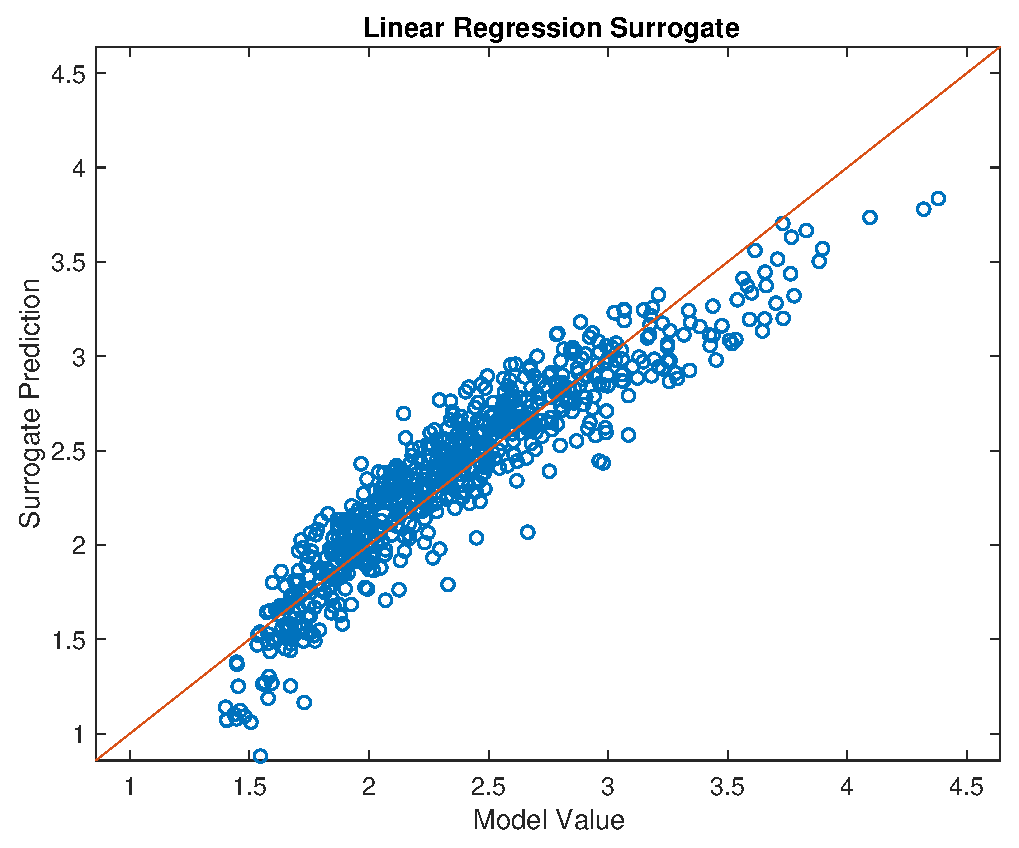
\includegraphics[width=.49 \textwidth]{Figures/Vol_Flow_QoI_LR_Prediction_Rectangular.eps}
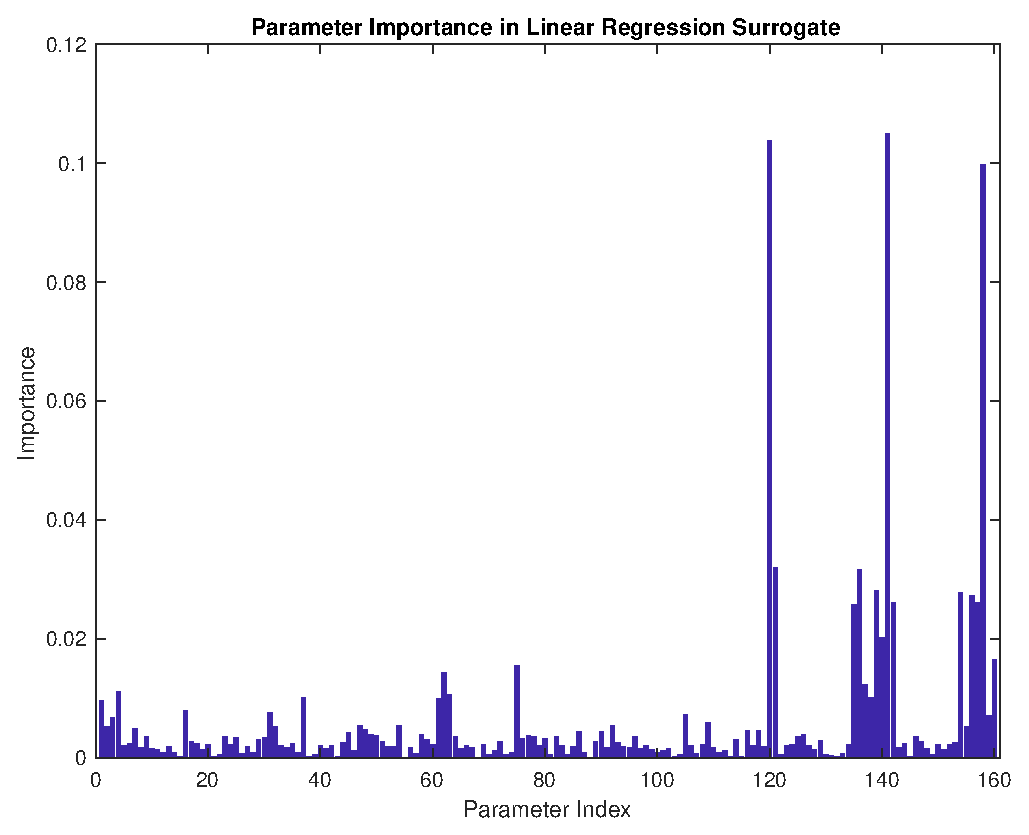
\includegraphics[width=.49 \textwidth]{Figures/Vol_Flow_QoI_LR_VI_Rectangular.eps}\\
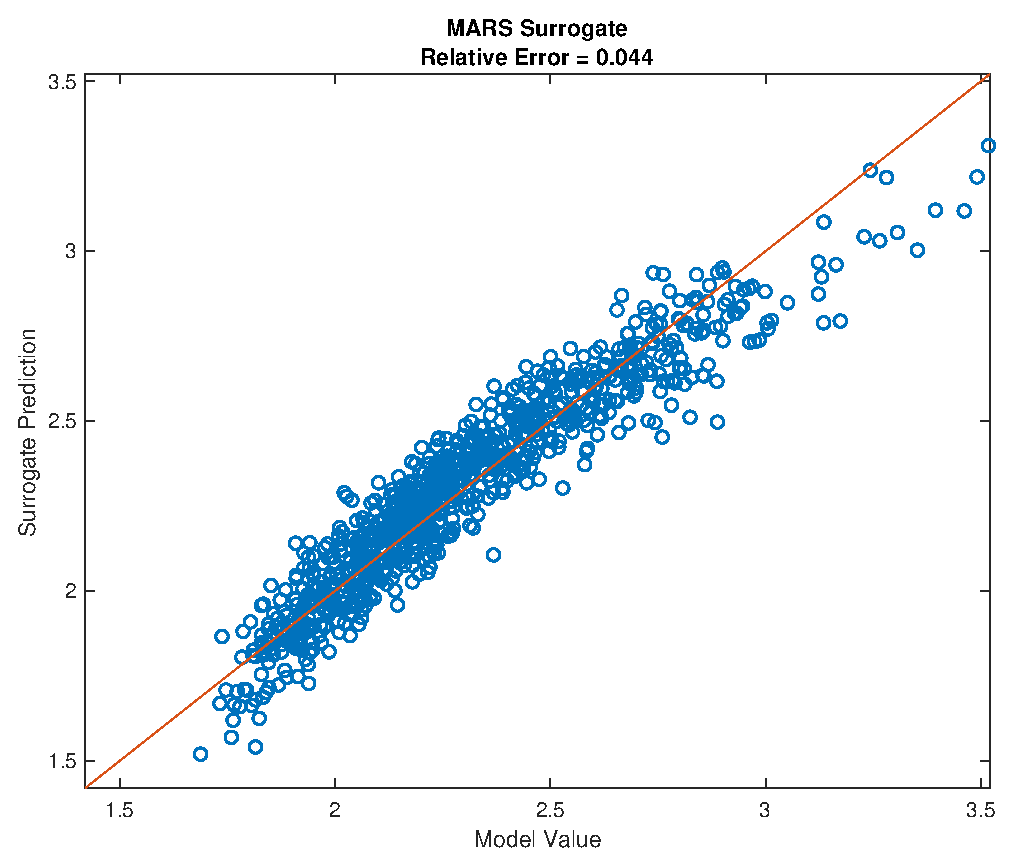
\includegraphics[width=.49 \textwidth]{Figures/Vol_Flow_QoI_MARS_Prediction_Rectangular.eps}
\includegraphics[width=.49 \textwidth]{Figures/Vol_Flow_QoI_MARS_VI_Rectangular.eps}
\end{figure}

Tabular data in Table~\ref{qoi_vol_flow_rec}.

\begin{table}[h]
\centering
\begin{tabular}{ccccc}
Index & Identification & LR Importance & MARS Importance & MARS Ranking \\
   120 & 5.5 in Buff\_e ODE & 0.1755 & 0.0612 & 3\\
   141 & z\_4 in SMCEC &  0.0955 & 0.3226 & 1\\
   158 & n\_cross in WallMechanics & 0.0903 & 0.2854 & 2\\
   121 & 1.09 in Buff\_e ODE & 0.0552 & 0.0311 & 7\\
   139 & z\_2 in SMCEC & 0.0326 & 0.0495 & 4\\
   136 & G\_K\_i in SMCEC & 0.0313 & 0.0412 & 6\\
   142 & z\_5 in SMCEC & 0.0295 & 0.0418 & 5\\
   135 & F\_NaK\_i in SMCEC & 0.0247 & 0.0244 & 11\\
   156 & K\_7 in WallMechanics & 0.0247 & 0.0284 & 8\\
   157 & gamma\_cross in WallMechanics & 0.0229 & 0.0275 & 9
\end{tabular}
\caption{(volumetric flow rate rectangular pulse stimulus) The importance of the parameters is assessed in two ways; ``LR Importance" is the absolute value of the linear regression coefficient normalized so that the sum of all indices equals 1 and ``MARS Importance" is delGCV measure build in MARS normalized so that the sum of all indices equals 1. The parameters are ordered according to the results from linear regression and the ordering of parameters by MARS is given in the ``MARS Ranking" column. The ``Index" column is indexing of the parameters in the code (primarily for Joey's use) and the ``Identification column" is the description of the parameter.}
\label{qoi_vol_flow_rec}
\end{table}

\newpage

\subsubsection{Experimental Data Stimulus}

\begin{figure}[h]
\centering
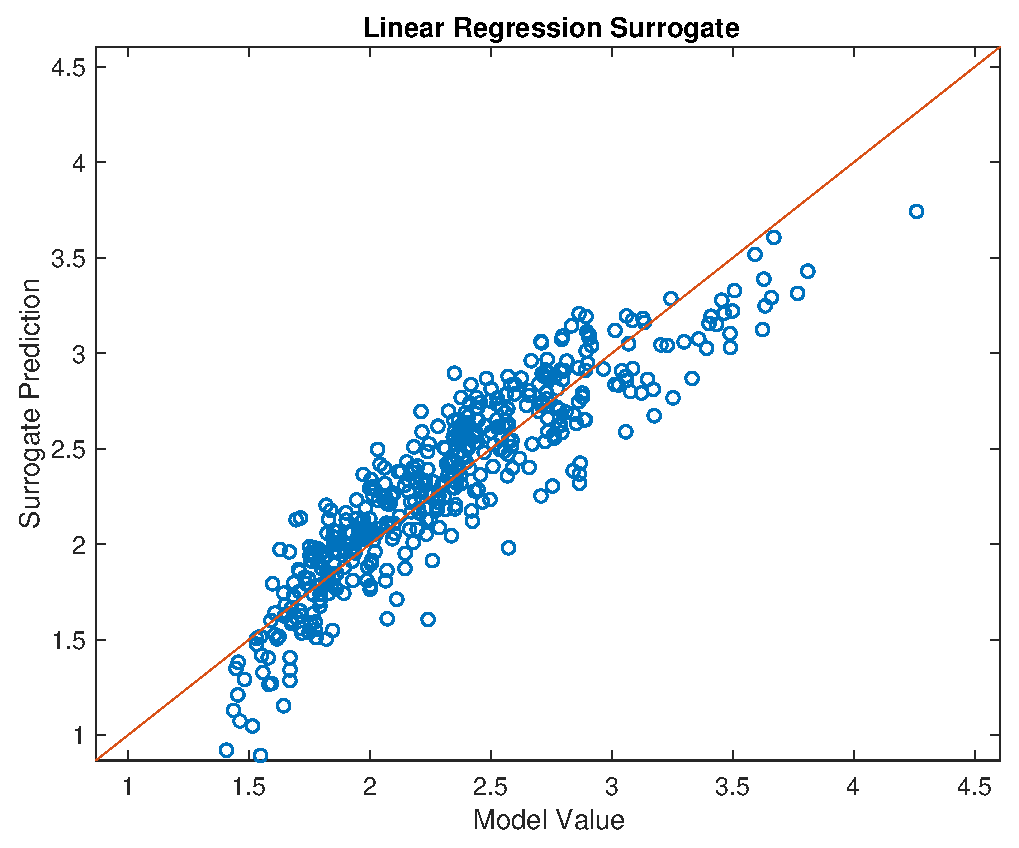
\includegraphics[width=.49 \textwidth]{Figures/Vol_Flow_QoI_LR_Prediction_Experimental.eps}
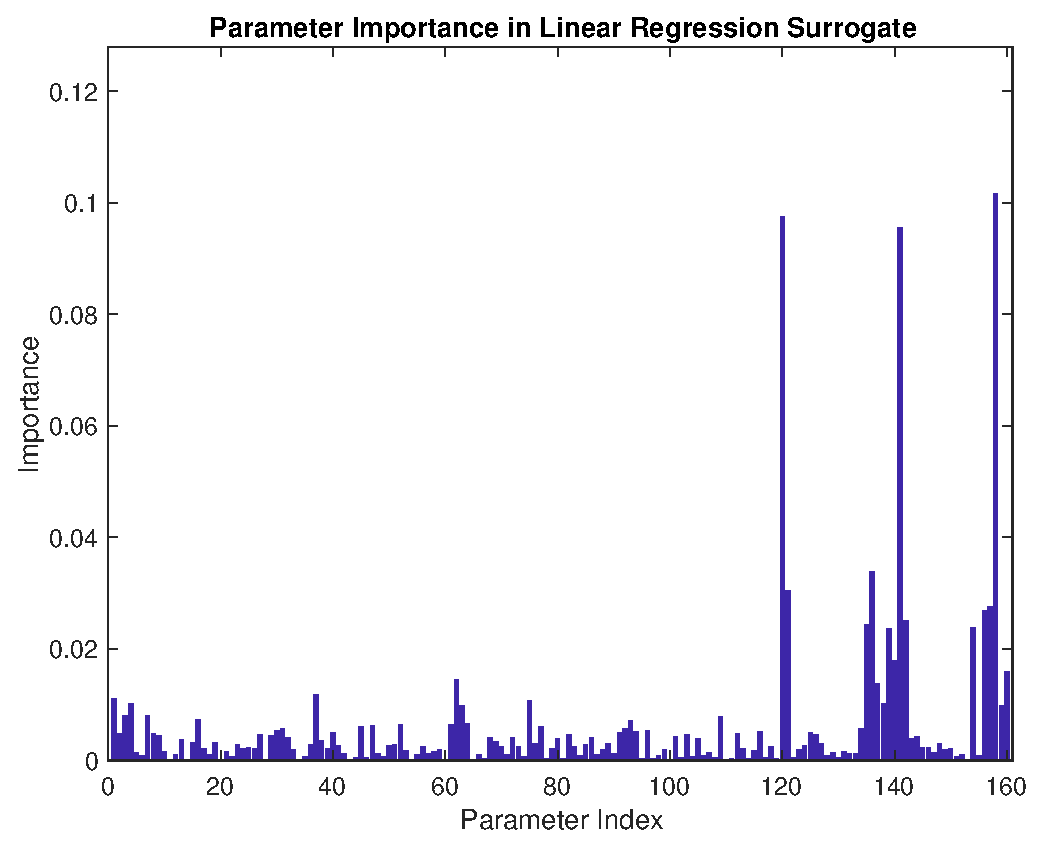
\includegraphics[width=.49 \textwidth]{Figures/Vol_Flow_QoI_LR_VI_Experimental.eps}\\
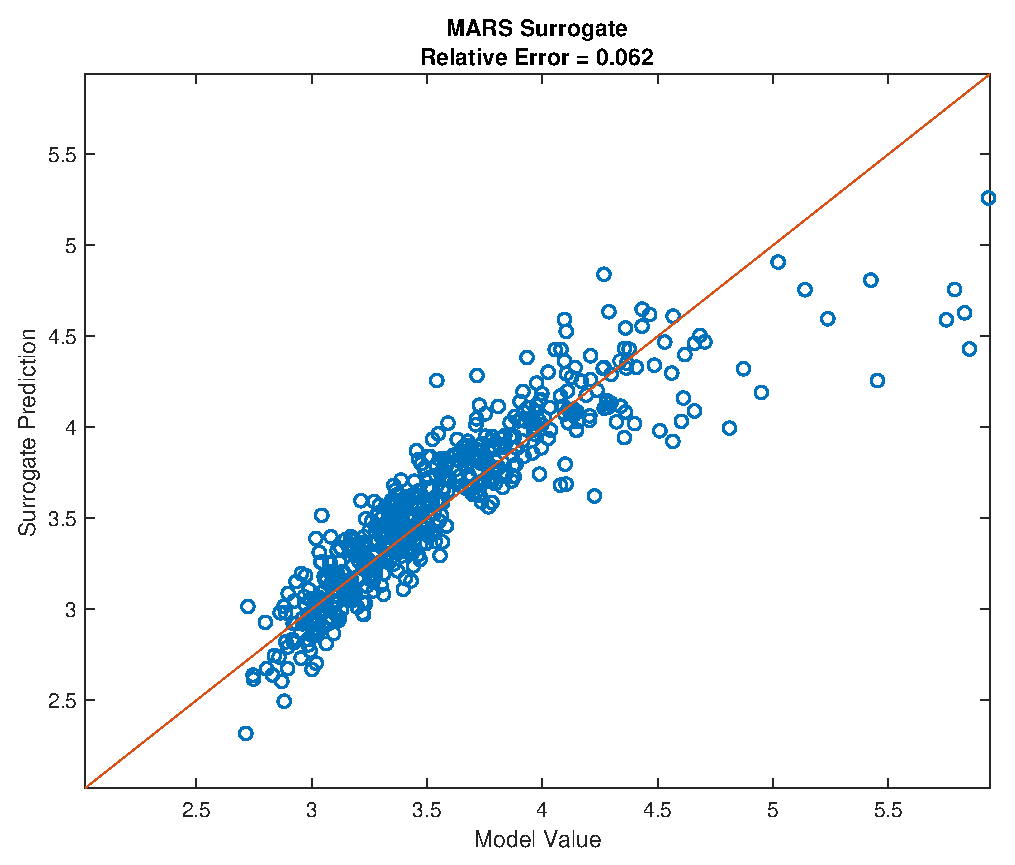
\includegraphics[width=.49 \textwidth]{Figures/Vol_Flow_QoI_MARS_Prediction_Experimental.eps}
\includegraphics[width=.49 \textwidth]{Figures/Vol_Flow_QoI_MARS_VI_Experimental.eps}
\end{figure}

Tabular data in Table~\ref{qoi_vol_flow_ex}.

\begin{table}[h]
\centering
\begin{tabular}{ccccc}
Index & Identification & LR Importance & MARS Importance & MARS Ranking \\
   120 & 5.5 in Buff\_e ODE & 0.1663 & 0.0626 & 3\\
   158 & n\_cross in WallMechanics  & 0.0755 & 0.3309 & 1\\
   141 & z\_4 in SMCEC & 0.0729 & 0.3270 & 2\\
   121 & 1.09 in Buff\_e ODE & 0.0490 & 0.0423 & 4\\
   136 & G\_K\_i in SMCEC & 0.0252 & 0.0335 & 6\\
   139 & z\_2 in SMCEC & 0.0239 & 0.0382 & 5\\
   142 & z\_5 in SMCEC & 0.0237 & 0.0285 & 7\\
   135 & F\_NaK\_i in SMCEC & 0.0229 & 0.0212 & 10\\
   156 & K\_7 in WallMechanics & 0.0190 & 0.0212 & 11\\
   140 & z\_3 in SMCEC & 0.0186 & 0.0266 & 8\\
\end{tabular}
\caption{(volumetric flow rate experimental data stimulus) The importance of the parameters is assessed in two ways; ``LR Importance" is the absolute value of the linear regression coefficient normalized so that the sum of all indices equals 1 and ``MARS Importance" is delGCV measure build in MARS normalized so that the sum of all indices equals 1. The parameters are ordered according to the results from linear regression and the ordering of parameters by MARS is given in the ``MARS Ranking" column. The ``Index" column is indexing of the parameters in the code (primarily for Joey's use) and the ``Identification column" is the description of the parameter.}
\label{qoi_vol_flow_ex}
\end{table}

\newpage

\subsection{QoI \eqref{K_ECS_Max} ($K_{ECS}$ Max)}

\subsubsection{Rectangular Pulse Stimulus}

\begin{figure}[h]
\centering
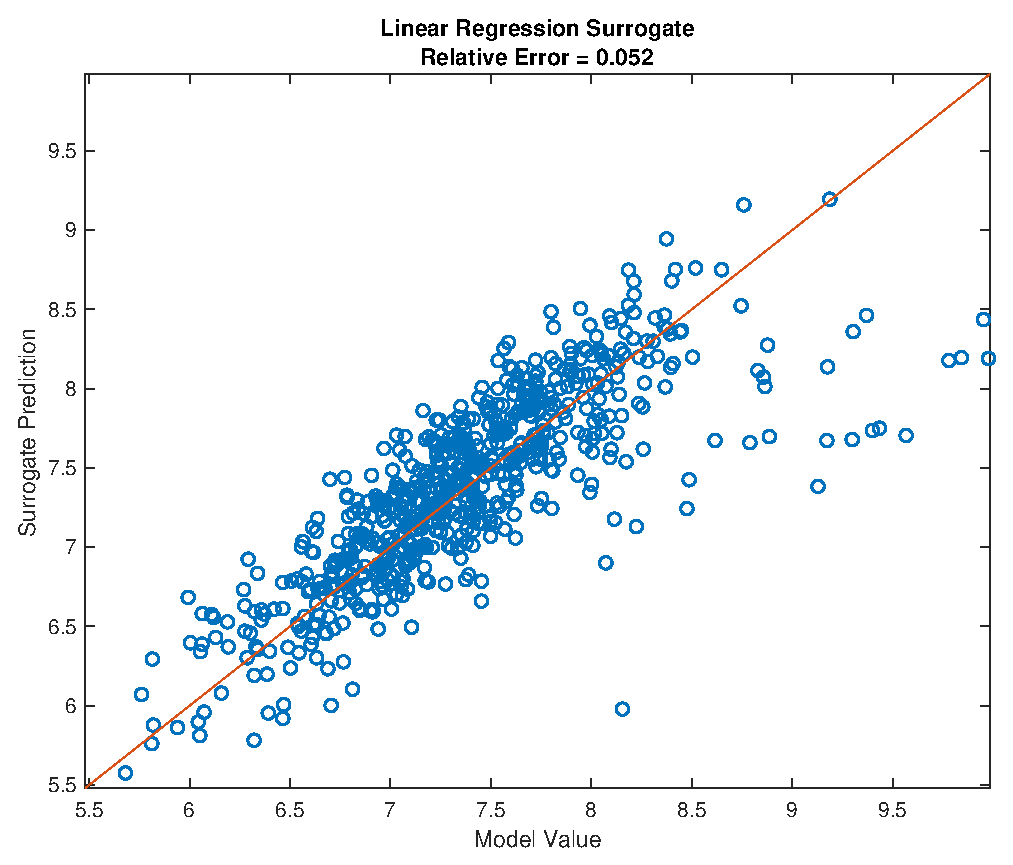
\includegraphics[width=.49 \textwidth]{Figures/K_ECS_Max_QoI_LR_Prediction_Rectangular.eps}
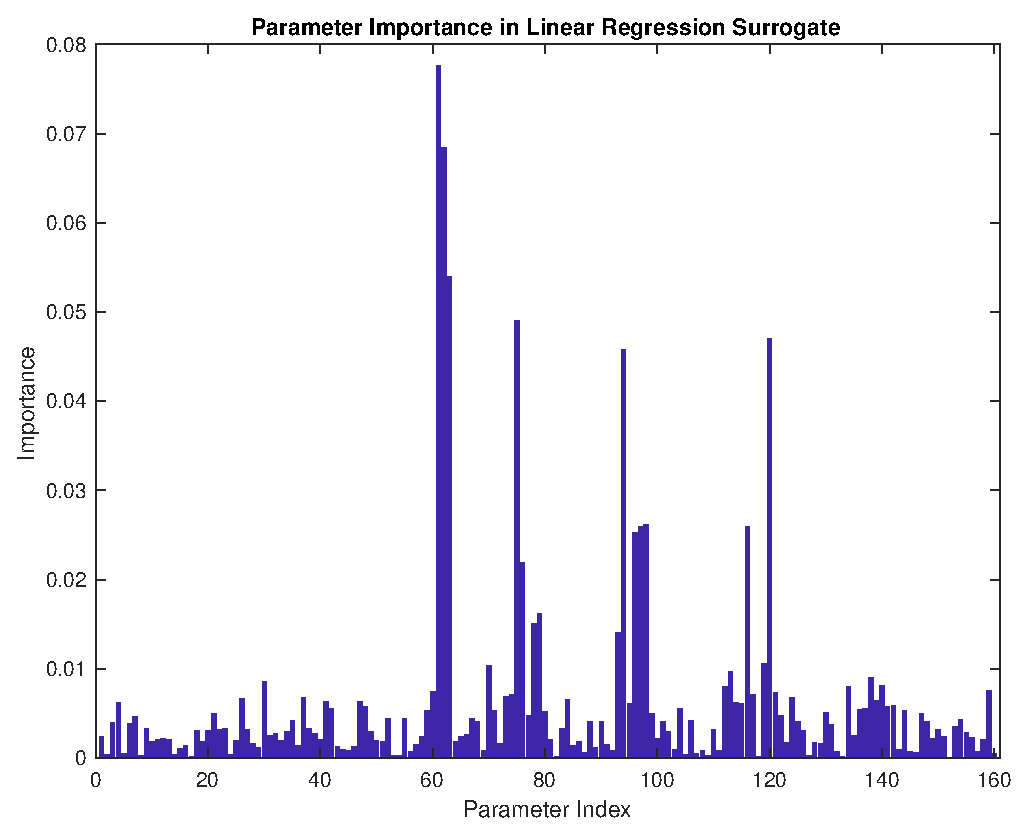
\includegraphics[width=.49 \textwidth]{Figures/K_ECS_Max_QoI_LR_VI_Rectangular.eps}\\
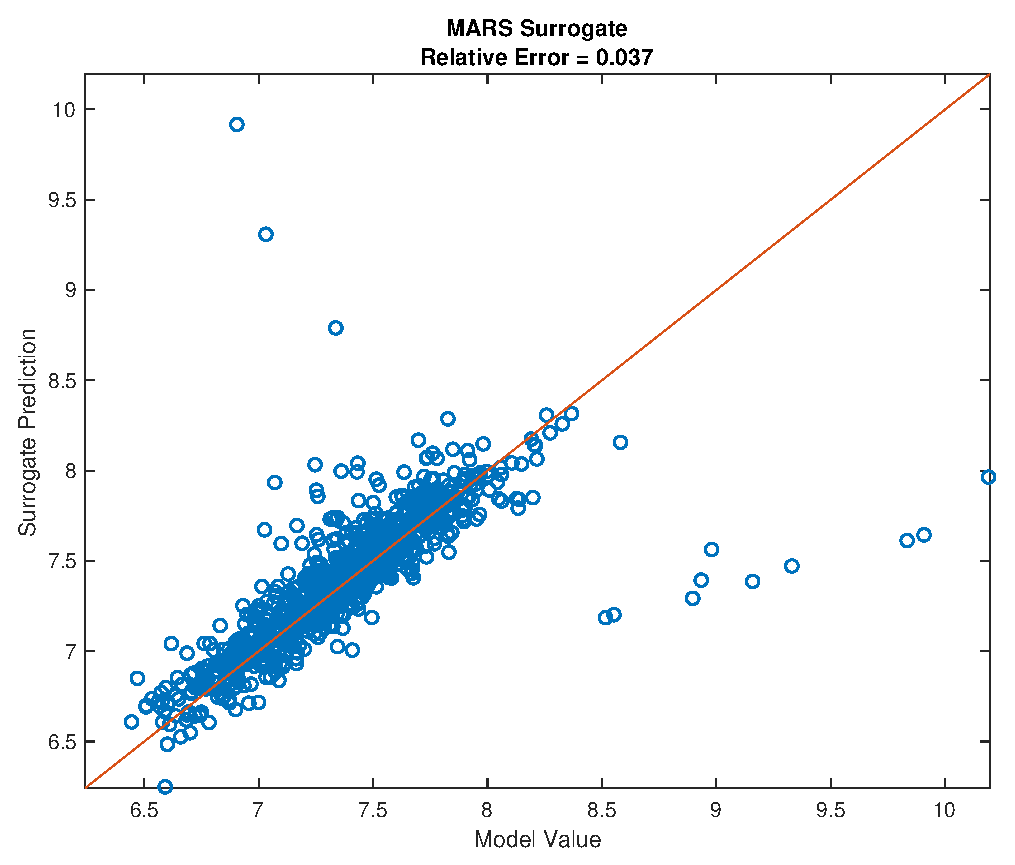
\includegraphics[width=.49 \textwidth]{Figures/K_ECS_Max_QoI_MARS_Prediction_Rectangular.eps}
\includegraphics[width=.49 \textwidth]{Figures/K_ECS_Max_QoI_MARS_VI_Rectangular.eps}
\end{figure}

Tabular data in Table~\ref{qoi_K_ECS_Max_rec}.

\begin{table}[h]
\centering
\begin{tabular}{ccccc}
Index & Identification & LR Importance & MARS Importance & MARS Ranking \\

61 & gKleak\_d in Neuron & 0.0752 &  0.2037 & 2\\
62 & 0.143 in m4alpha and m4 beta & 0.0742 & 0.2218 & 1\\
120 & 5.5 in Buff\_e ODE & 0.0641 & 0 & none\\
63 &   5.67 in m4alpha and m4 beta & 0.0631 & 0.1673 & 3\\
75 & 34.9 in m6alpha & 0.0570 & 0.1349 & 4\\
116 & dhod in Neuron & 0.0299 & 0.0802 & 5\\
94 & 34.9 in m2alpha & 0.0295 & 0.0647 & 6\\
76 & 0.2 in m6alpha & 0.0284 & 0.0317 &7\\
97 & 0.025 in m2beta & 0.0252 & 0.0097 & 12\\
98 & 1.25 in m2beta & 0.0239 & 0.0203 & 10\\
\end{tabular}
\caption{ ($K_{ECS}$ Max rectangular pulse stimulus) The importance of the parameters is assessed in two ways; ``LR Importance" is the absolute value of the linear regression coefficient normalized so that the sum of all indices equals 1 and ``MARS Importance" is delGCV measure build in MARS normalized so that the sum of all indices equals 1. The parameters are ordered according to the results from linear regression and the ordering of parameters by MARS is given in the ``MARS Ranking" column. The ``Index" column is indexing of the parameters in the code (primarily for Joey's use) and the ``Identification column" is the description of the parameter.}
\label{qoi_K_ECS_Max_rec}
\end{table}

\newpage

\subsubsection{Experimental Data Stimulus}

\begin{figure}[h]
\centering
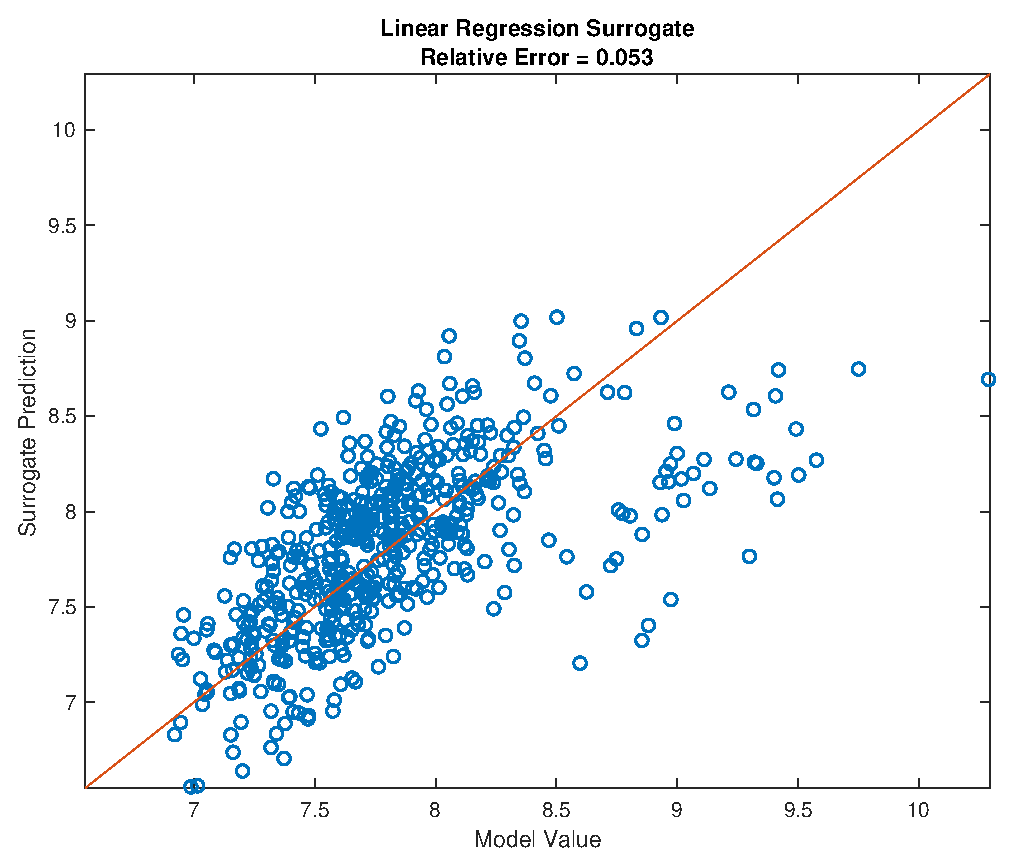
\includegraphics[width=.49 \textwidth]{Figures/K_ECS_Max_QoI_LR_Prediction_Experimental.eps}
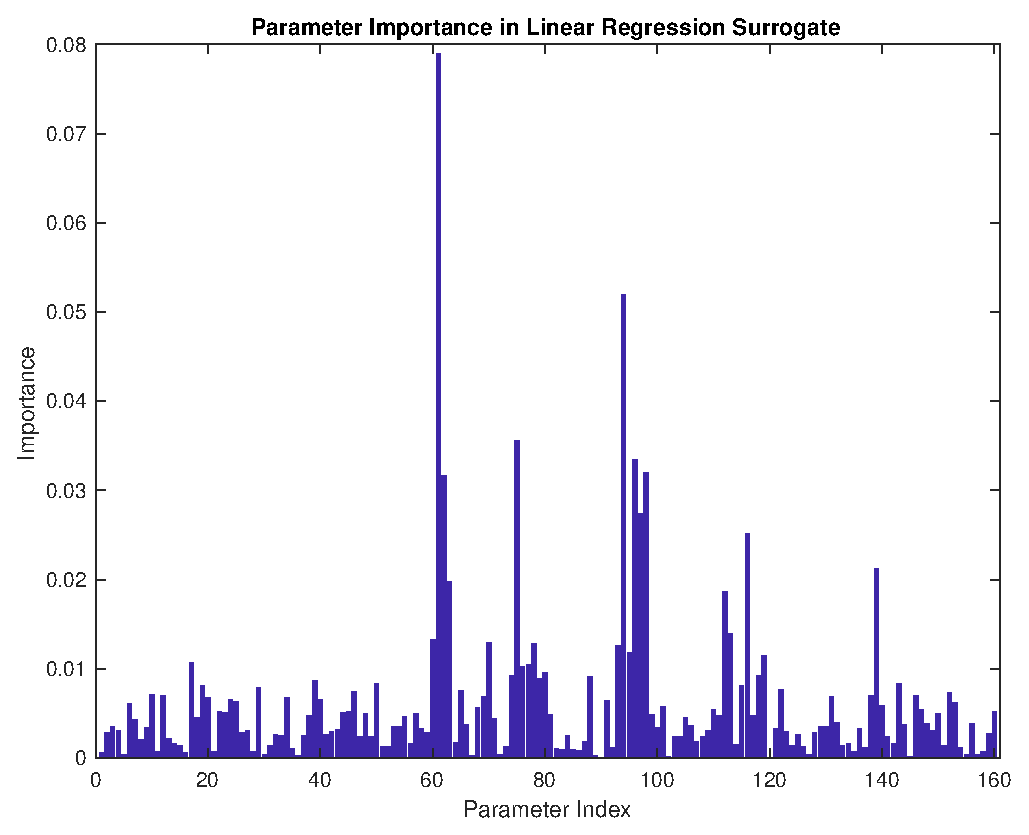
\includegraphics[width=.49 \textwidth]{Figures/K_ECS_Max_QoI_LR_VI_Experimental.eps}\\
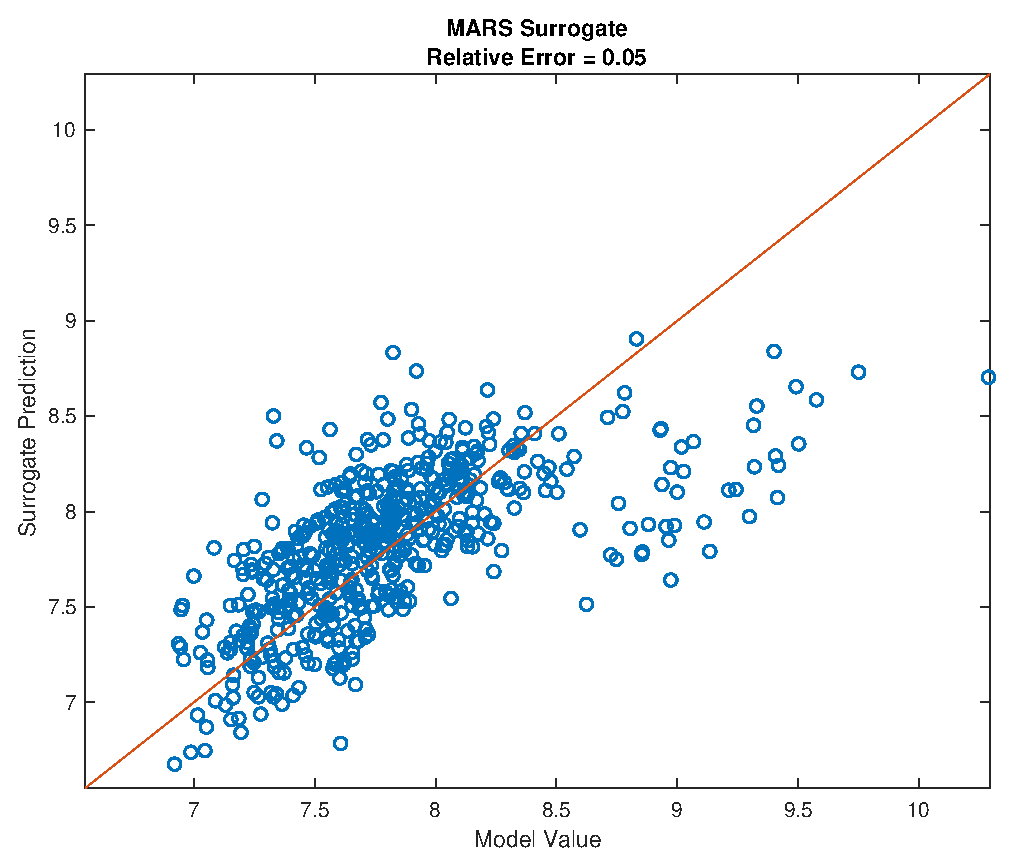
\includegraphics[width=.49 \textwidth]{Figures/K_ECS_Max_QoI_MARS_Prediction_Experimental.eps}
\includegraphics[width=.49 \textwidth]{Figures/K_ECS_Max_QoI_MARS_VI_Experimental.eps}
\end{figure}

Tabular data in Table~\ref{qoi_K_ECS_Max_ex}.

\begin{table}[h]
\centering
\begin{tabular}{ccccc}
Index & Identification & LR Importance & MARS Importance & MARS Ranking \\
120 & 5.5 in Buff\_e ODE & 0.1099 & 0 & none\\
94 & 34.9 in m2alpha & 0.0740 & 0.2584 & 2\\
61 & gKleak\_d in Neuron & 0.0590 &  0.3023 & 1\\ 
121 & 1.09 in Buff\_e ODE & 0.0487 & 0 &  none\\
98 & 1.25 in m2beta & 0.0341 &  0.0698 & 3\\
97 & 0.025 in m2beta & 0.0258 & 0.0547 & 7\\
96 & 0.25 in m2beta & 0.0243 &  0.0624 & 6\\
93 & 0.016 in m2alpha & 0.0241 & 0.0670 & 4\\
75 & 34.9 in m6alpha & 0.0187 & 0.0349 & 8\\
119 & B0 & 0.0161 & 0 & none
\end{tabular}
\caption{ ($K_{ECS}$ Max experimental data stimulus) The importance of the parameters is assessed in two ways; ``LR Importance" is the absolute value of the linear regression coefficient normalized so that the sum of all indices equals 1 and ``MARS Importance" is delGCV measure build in MARS normalized so that the sum of all indices equals 1. The parameters are ordered according to the results from linear regression and the ordering of parameters by MARS is given in the ``MARS Ranking" column. The ``Index" column is indexing of the parameters in the code (primarily for Joey's use) and the ``Identification column" is the description of the parameter.}
\label{qoi_K_ECS_Max_ex}
\end{table}


\newpage
\subsection{QoI \eqref{K_ECS_Mean} ($K_{ECS}$ Mean)}

\subsubsection{Rectangular Pulse Stimulus}

\begin{figure}[h]
\centering
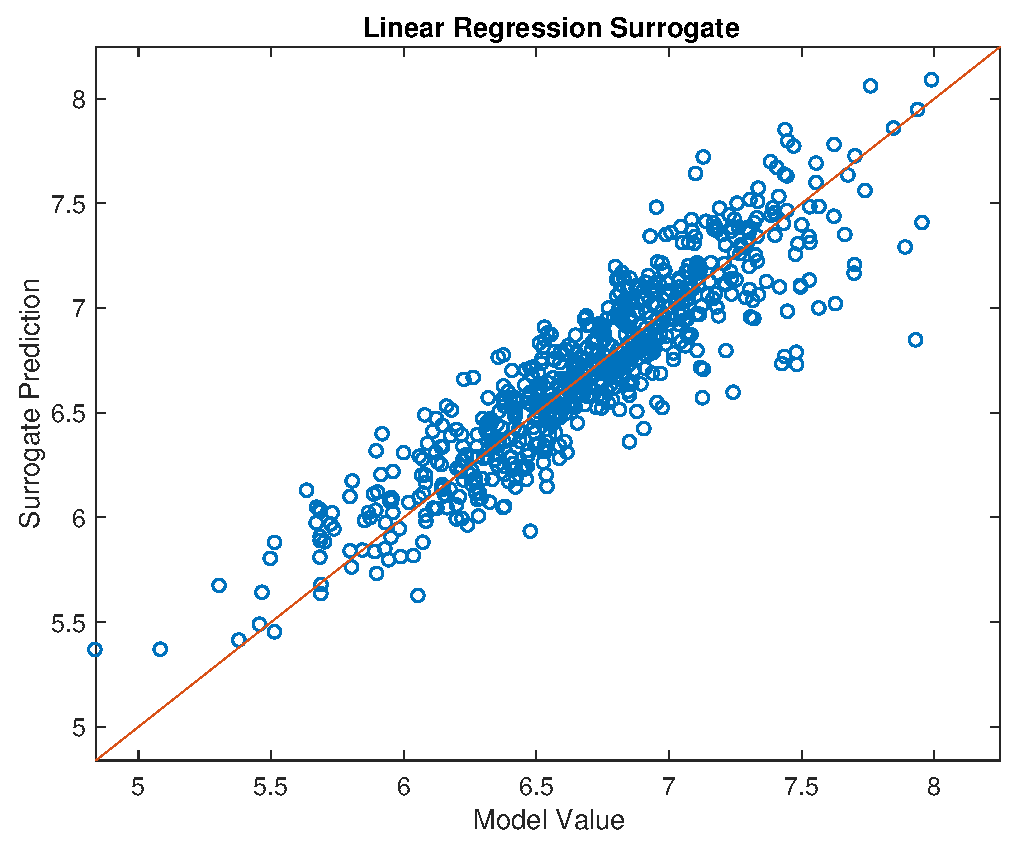
\includegraphics[width=.49 \textwidth]{Figures/K_ECS_Mean_QoI_LR_Prediction_Rectangular.eps}
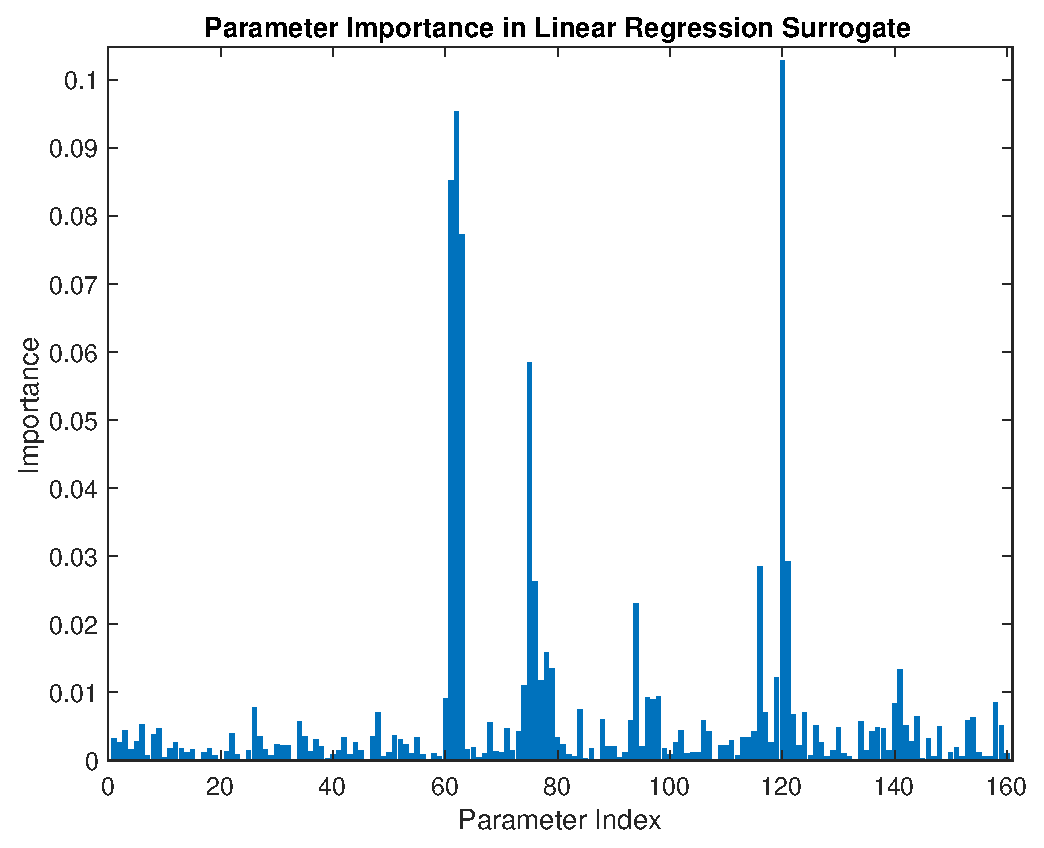
\includegraphics[width=.49 \textwidth]{Figures/K_ECS_Mean_QoI_LR_VI_Rectangular.eps}\\
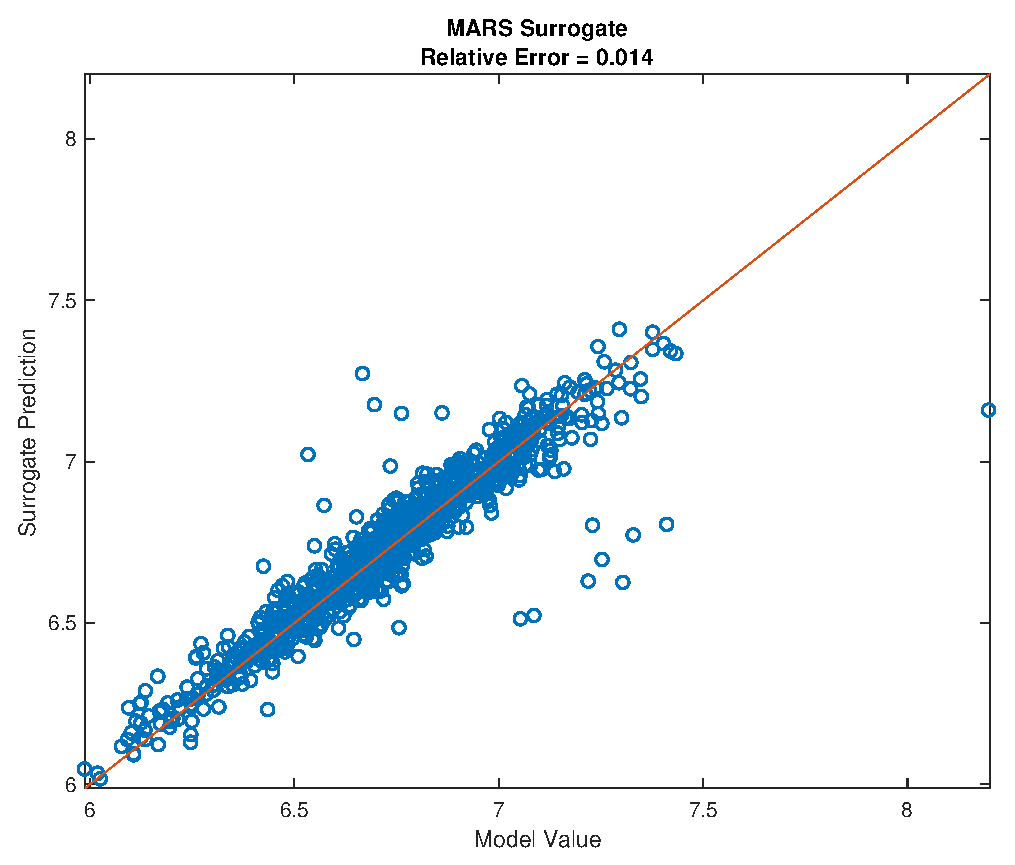
\includegraphics[width=.49 \textwidth]{Figures/K_ECS_Mean_QoI_MARS_Prediction_Rectangular.eps}
\includegraphics[width=.49 \textwidth]{Figures/K_ECS_Mean_QoI_MARS_VI_Rectangular.eps}
\end{figure}

Tabular data in Table~\ref{qoi_K_ECS_Mean_rec}.

\begin{table}[h]
\centering
\begin{tabular}{ccccc}
Index & Identification & LR Importance & MARS Importance & MARS Ranking \\
62 & 0.143 in m4alpha and m4 beta &  0.1078 & 0.2854 & 1\\
61 & gKleak\_d in Neuron & 0.0912 & 0.2117 & 2\\
120 & 5.5 in Buff\_e ODE & 0.0906 & 0.0107 & 10\\
63 &   5.67 in m4alpha and m4 beta & 0.0878 & 0.2088 & 3\\
75 & 34.9 in m6alpha & 0.0691 & 0.1320 & 4\\
116 & dhod in Neuron & 0.0372 & 0.0409 & 5\\
76 & 0.2 in m6alpha & 0.0335 & 0.0380 & 6\\
121 & 1.09 in Buff\_e ODE & 0.0249 & none & \\
74 & 0.016 in m6alpha & 0.0188 & 0.0114 & 9\\
78 & 0.025 in m6beta & 0.0186 & 0.0079 & 13\\
\end{tabular}
\caption{($K_{ECS}$ Mean rectangular pulse stimulus) The importance of the parameters is assessed in two ways; ``LR Importance" is the absolute value of the linear regression coefficient normalized so that the sum of all indices equals 1 and ``MARS Importance" is delGCV measure build in MARS normalized so that the sum of all indices equals 1. The parameters are ordered according to the results from linear regression and the ordering of parameters by MARS is given in the ``MARS Ranking" column. The ``Index" column is indexing of the parameters in the code (primarily for Joey's use) and the ``Identification column" is the description of the parameter.}
\label{qoi_K_ECS_Mean_rec}
\end{table}

\newpage

\subsubsection{Experimental Data Stimulus}

\begin{figure}[h]
\centering
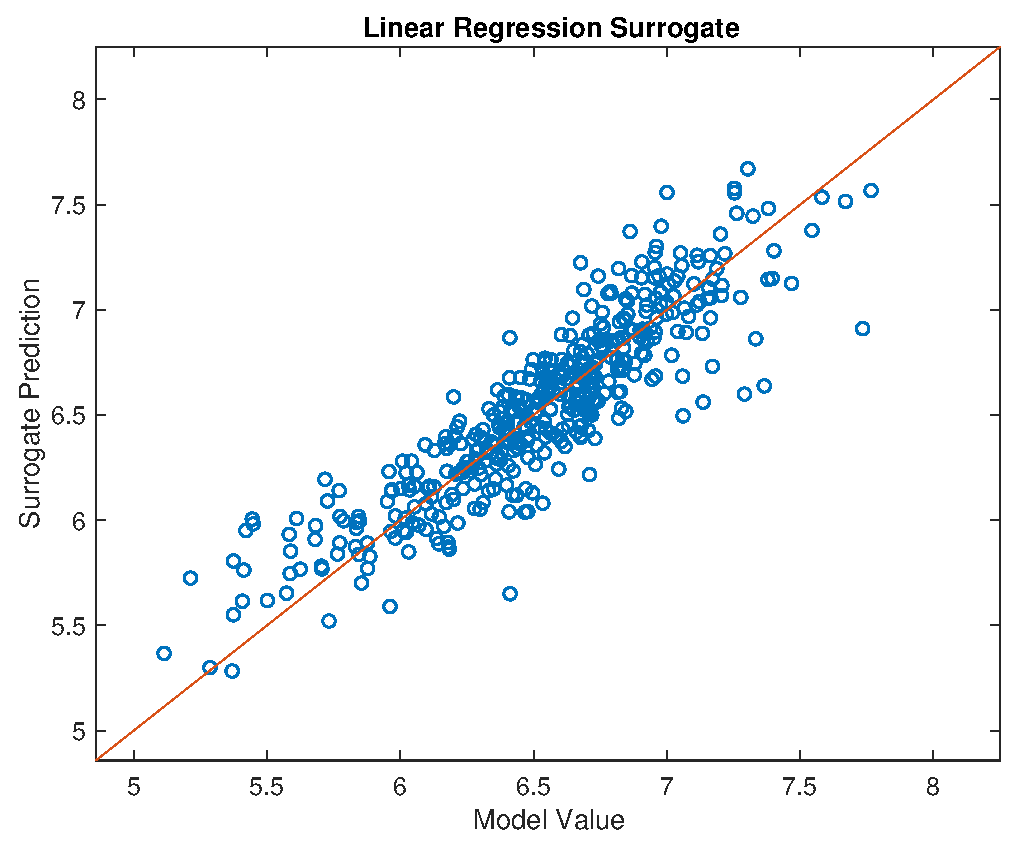
\includegraphics[width=.49 \textwidth]{Figures/K_ECS_Mean_QoI_LR_Prediction_Experimental.eps}
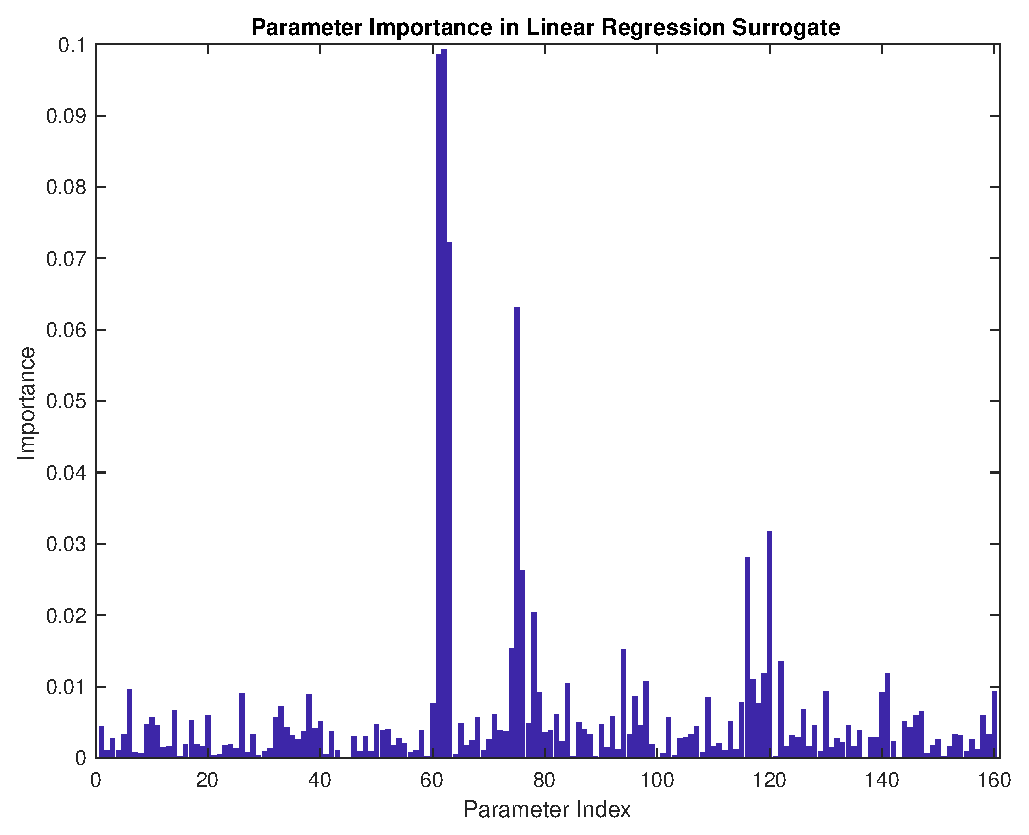
\includegraphics[width=.49 \textwidth]{Figures/K_ECS_Mean_QoI_LR_VI_Experimental.eps}\\
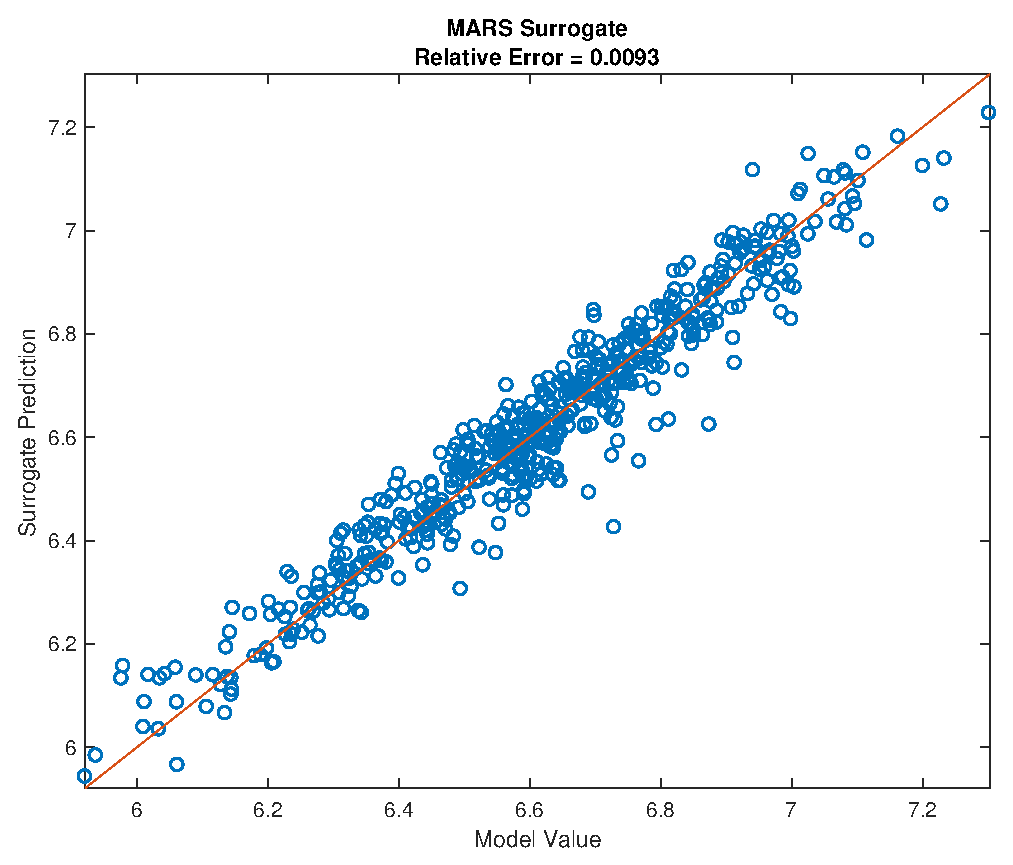
\includegraphics[width=.49 \textwidth]{Figures/K_ECS_Mean_QoI_MARS_Prediction_Experimental.eps}
\includegraphics[width=.49 \textwidth]{Figures/K_ECS_Mean_QoI_MARS_VI_Experimental.eps}
\end{figure}

Tabular data in Table~\ref{qoi_K_ECS_Mean_ex}.


\begin{table}[h]
\centering
\begin{tabular}{ccccc}
Index & Identification & LR Importance & MARS Importance & MARS Ranking \\
62 & 0.143 in m4alpha and m4 beta &  0.1043 & 0.2817 & 1\\
61 & gKleak\_d in Neuron & 0.0954 & 0.2357 &  2\\
63 &   5.67 in m4alpha and m4 beta & 0.0827 & 0.1929 & 3\\
120 & 5.5 in Buff\_e ODE & 0.0781 & 0.0105 & 10\\
75 & 34.9 in m6alpha & 0.0648 & 0.1232 & 4\\
76 & 0.2 in m6alpha & 0.0349 & 0.0473 & 5\\
116 & dhod in Neuron & 0.0331 & 0.0040 & 6\\
121 & 1.09 in Buff\_e ODE & 0.0227 & 0.0040 & 14\\
78 & 0.025 in m6beta & 0.0183 &  0.0065 & 13\\
79 & 1.25 in m6beta & 0.0168 & 0.0110 & 9\\
\end{tabular}
\caption{($K_{ECS}$ Mean experimental data stimulus) The importance of the parameters is assessed in two ways; ``LR Importance" is the absolute value of the linear regression coefficient normalized so that the sum of all indices equals 1 and ``MARS Importance" is delGCV measure build in MARS normalized so that the sum of all indices equals 1. The parameters are ordered according to the results from linear regression and the ordering of parameters by MARS is given in the ``MARS Ranking" column. The ``Index" column is indexing of the parameters in the code (primarily for Joey's use) and the ``Identification column" is the description of the parameter.}
\label{qoi_K_ECS_Mean_ex}
\end{table}

\newpage
\subsection{QoI \eqref{K_AC_Max} ($K_{AC}$ Max)}

\subsubsection{Rectangular Pulse Stimulus}

\begin{figure}[h]
\centering
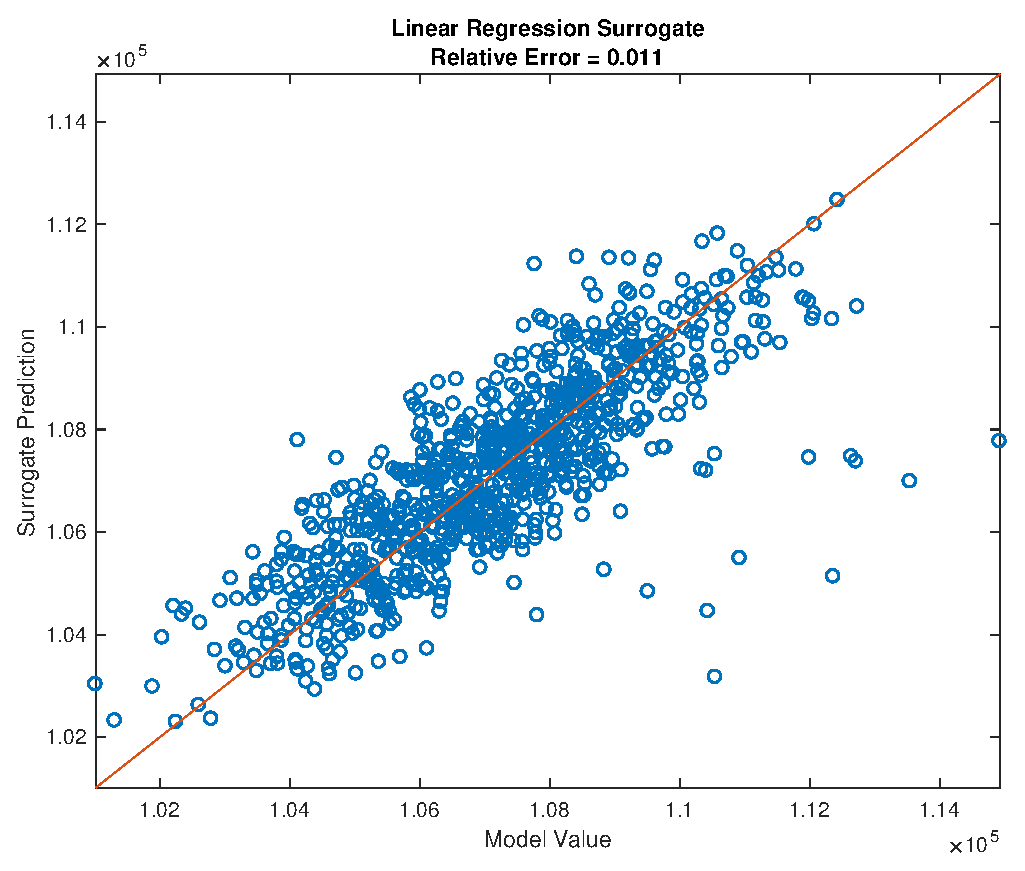
\includegraphics[width=.49 \textwidth]{Figures/K_AC_Max_QoI_LR_Prediction_Rectangular.eps}
\includegraphics[width=.49 \textwidth]{Figures/K_AC_Max_QoI_LR_VI_Rectangular.eps}\\
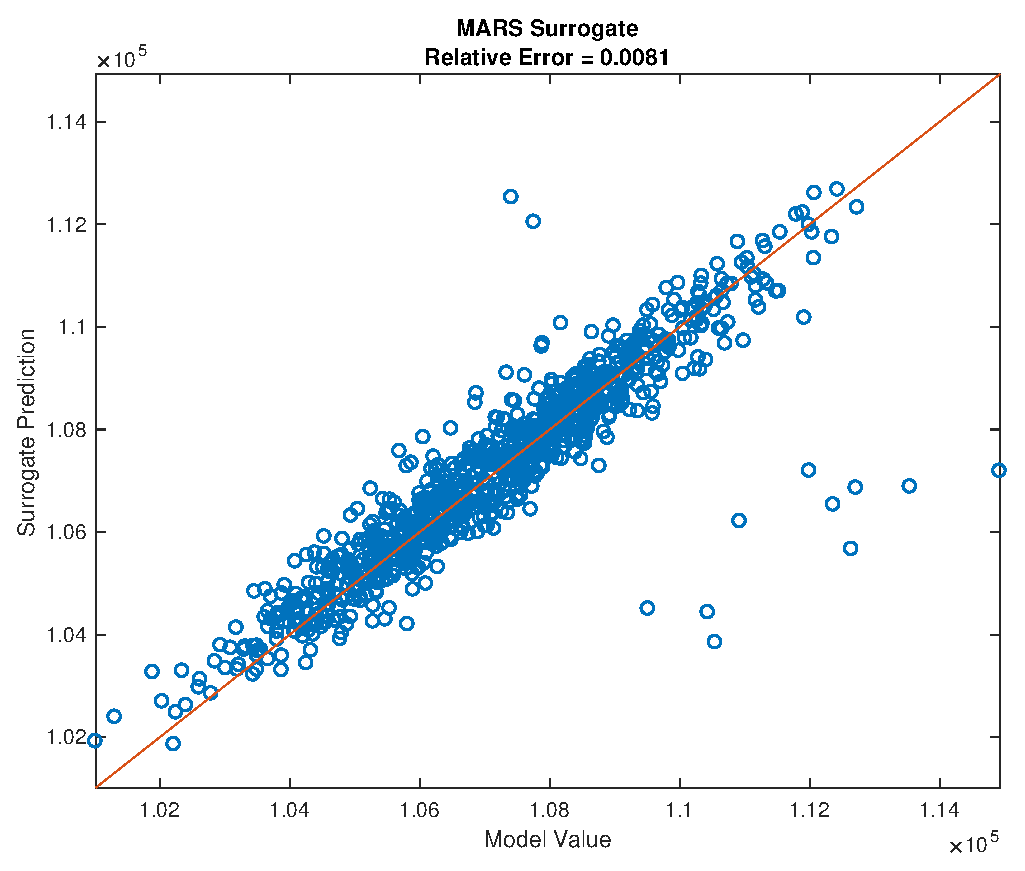
\includegraphics[width=.49 \textwidth]{Figures/K_AC_Max_QoI_MARS_Prediction_Rectangular.eps}
\includegraphics[width=.49 \textwidth]{Figures/K_AC_Max_QoI_MARS_VI_Rectangular.eps}
\end{figure}

Tabular data in Table~\ref{qoi_K_AC_Max_rec}.

\begin{table}[h]
\centering
\begin{tabular}{ccccc}
Index & Identification & LR Importance & MARS Importance & MARS Ranking \\
120 & 5.5 in Buff\_e ODE & 0.2455 & 0.3379 & 1\\
121 & 1.09 in Buff\_e ODE & 0.0749 & 0.2155 & 2\\
62 & 0.143 in m4alpha and m4 beta &  0.0362 & 0.1237 & 3\\
63 &   5.67 in m4alpha and m4 beta & 0.0286 & 0.0941 & 4\\
75 & 34.9 in m6alpha & 0.0285 & 0.0732 & 5\\
61 & gKleak\_d in Neuron & 0.0270 & 0.0595 & 6\\
97 & 0.025 in m2beta & 0.0126 & 0 & none\\
76 & 0.2 in m6alpha & 0.0117 &  0.0186 & 8\\
74 & 0.016 in m6alpha & 0.0106 & 0 & none\\
95 & 0.2 in m2alpha & 0.0104 & 0 & none\\
\end{tabular}
\caption{ ($K_{AC}$ Max rectangular pulse stimulus) The importance of the parameters is assessed in two ways; ``LR Importance" is the absolute value of the linear regression coefficient normalized so that the sum of all indices equals 1 and ``MARS Importance" is delGCV measure build in MARS normalized so that the sum of all indices equals 1. The parameters are ordered according to the results from linear regression and the ordering of parameters by MARS is given in the ``MARS Ranking" column. The ``Index" column is indexing of the parameters in the code (primarily for Joey's use) and the ``Identification column" is the description of the parameter.}
\label{qoi_K_AC_Max_rec}
\end{table}

\newpage

\subsubsection{Experimental Data Stimulus}

\begin{figure}[h]
\centering
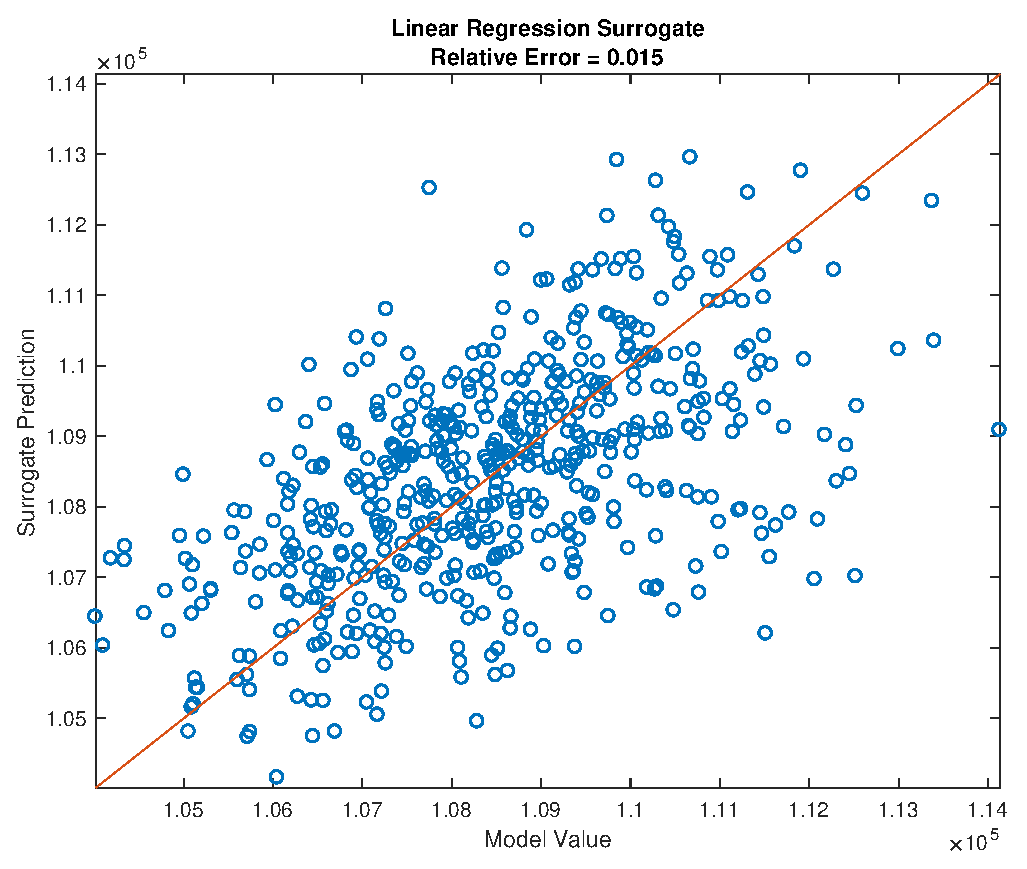
\includegraphics[width=.49 \textwidth]{Figures/K_AC_Max_QoI_LR_Prediction_Experimental.eps}
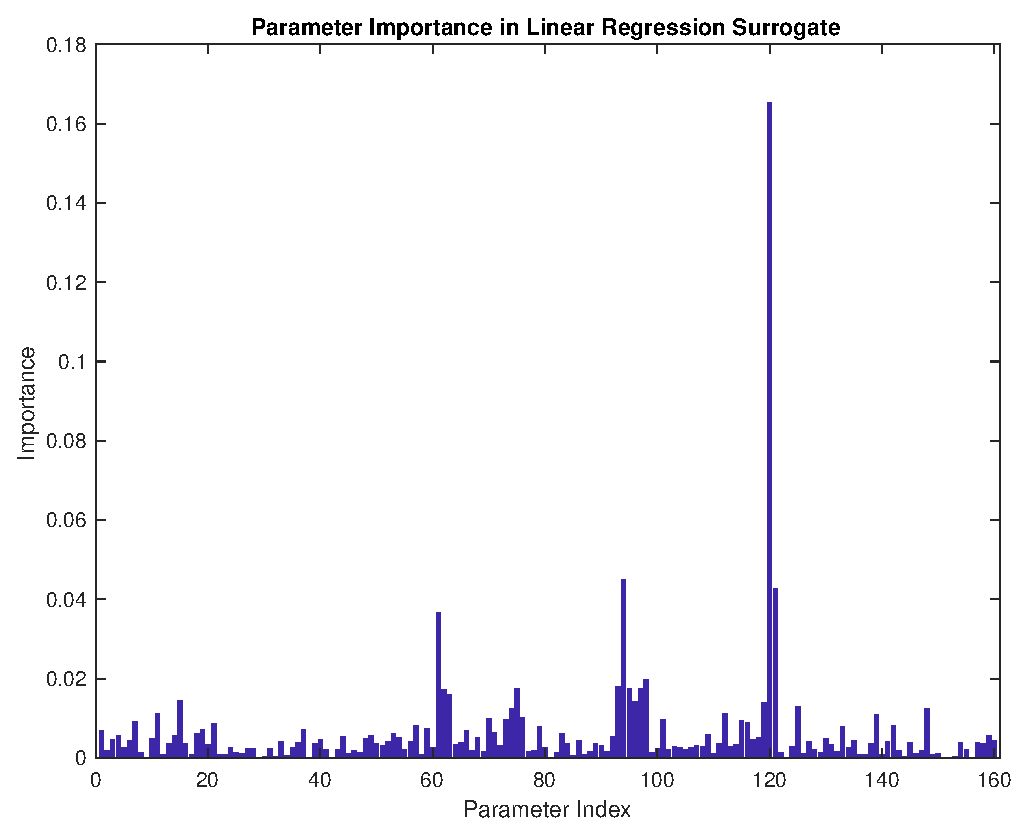
\includegraphics[width=.49 \textwidth]{Figures/K_AC_Max_QoI_LR_VI_Experimental.eps}\\
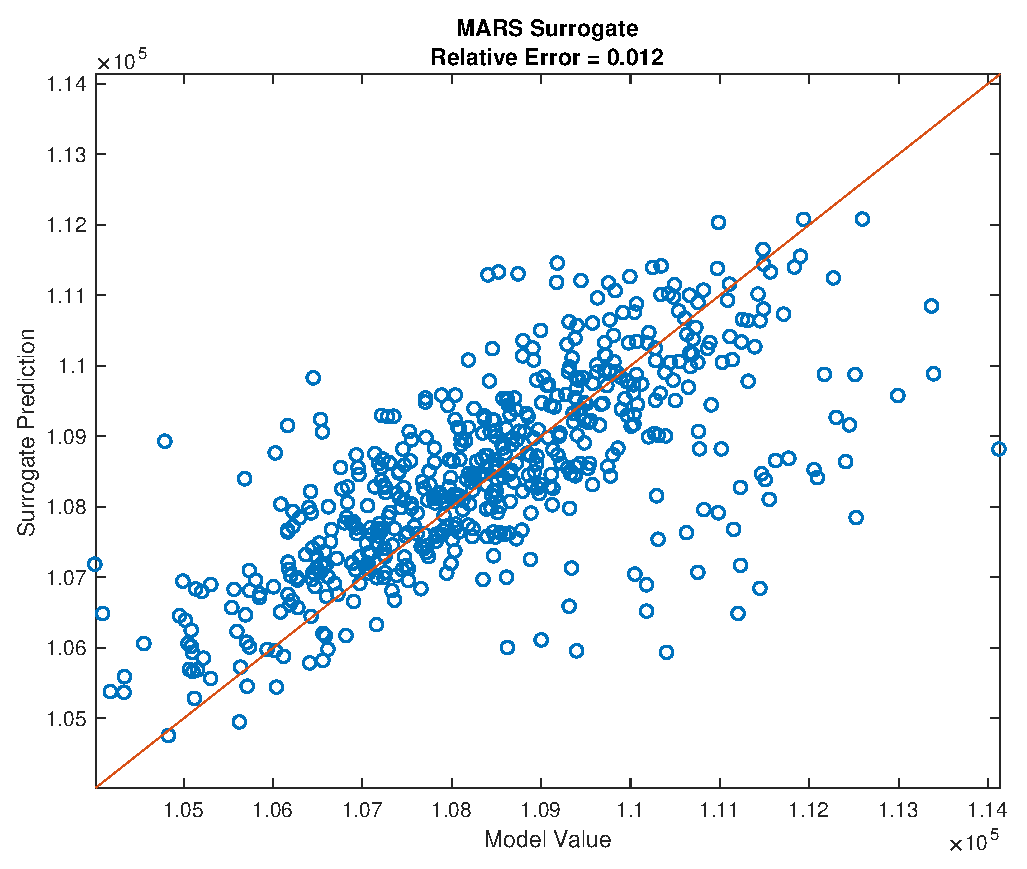
\includegraphics[width=.49 \textwidth]{Figures/K_AC_Max_QoI_MARS_Prediction_Experimental.eps}
\includegraphics[width=.49 \textwidth]{Figures/K_AC_Max_QoI_MARS_VI_Experimental.eps}
\end{figure}

Tabular data in Table~\ref{qoi_K_AC_Max_ex}.

\begin{table}[h]
\centering
\begin{tabular}{ccccc}
Index & Identification & LR Importance & MARS Importance & MARS Ranking \\
120 & 5.5 in Buff\_e ODE & 0.1654 & 0.2521 & 1\\
94 & 34.9 in m2alpha & 0.0450 & 0.1545 & 3\\
121 & 1.09 in Buff\_e ODE &  0.0427 & 0.2221 & 2\\
61 & gKleak\_d in Neuron & 0.0366 & 0.1032 & 4\\
98 & 1.25 in m2beta & 0.0197 & 0.0430 & 6\\
93 & 0.016 in m2alpha & 0.0180 & 0.0182 & 12\\
97 & 0.025 in m2beta & 0.0176 &  0 & none\\
75 & 34.9 in m6alpha & 0.0176 & 0.0470 & 5\\
95 & 0.2 in m2alpha & 0.0176 & 0 & none\\
62 & 0.143 in m4alpha and m4 beta &  0.0174 & 0.0329 & 8\\
\end{tabular}
\caption{ ($K_{AC}$ Max experimental data stimulus) The importance of the parameters is assessed in two ways; ``LR Importance" is the absolute value of the linear regression coefficient normalized so that the sum of all indices equals 1 and ``MARS Importance" is delGCV measure build in MARS normalized so that the sum of all indices equals 1. The parameters are ordered according to the results from linear regression and the ordering of parameters by MARS is given in the ``MARS Ranking" column. The ``Index" column is indexing of the parameters in the code (primarily for Joey's use) and the ``Identification column" is the description of the parameter.}
\label{qoi_K_AC_Max_ex}
\end{table}

\newpage
\subsection{QoI \eqref{K_AC_Mean}($K_{AC}$ Mean)}

\subsubsection{Rectangular Pulse Stimulus}

\begin{figure}[h]
\centering
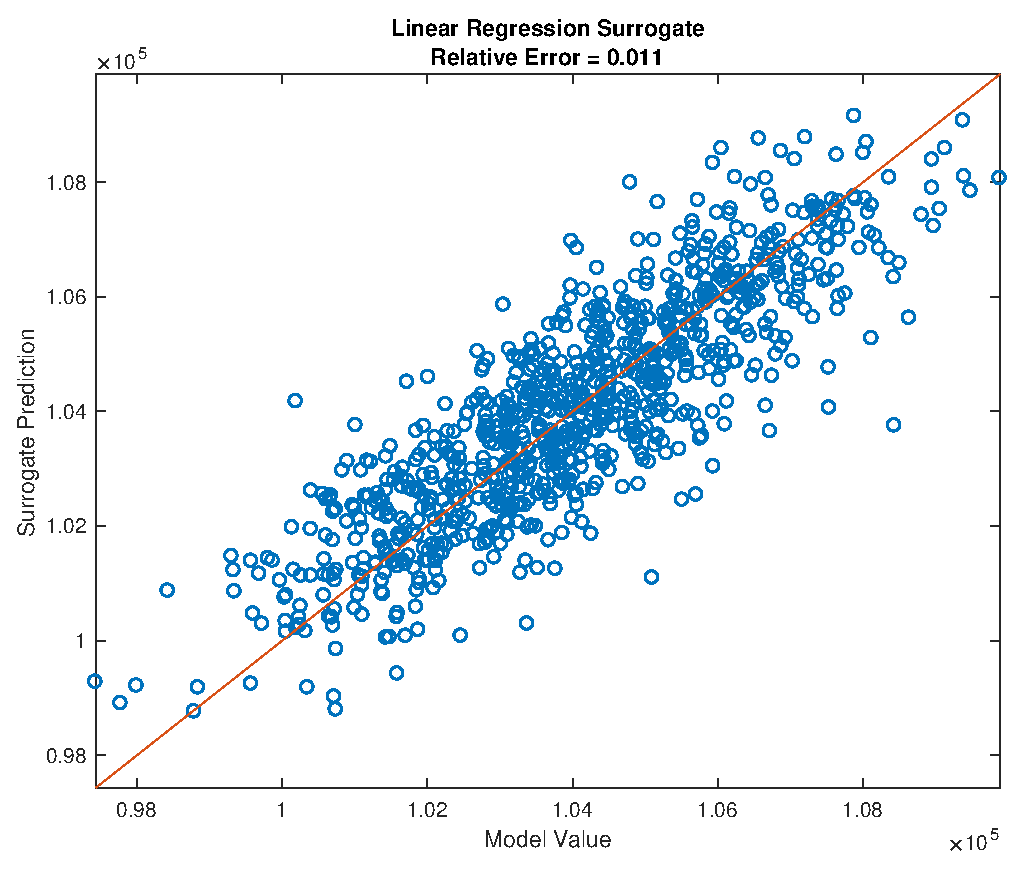
\includegraphics[width=.49 \textwidth]{Figures/K_AC_Mean_QoI_LR_Prediction_Rectangular.eps}
\includegraphics[width=.49 \textwidth]{Figures/K_AC_Mean_QoI_LR_VI_Rectangular.eps}\\
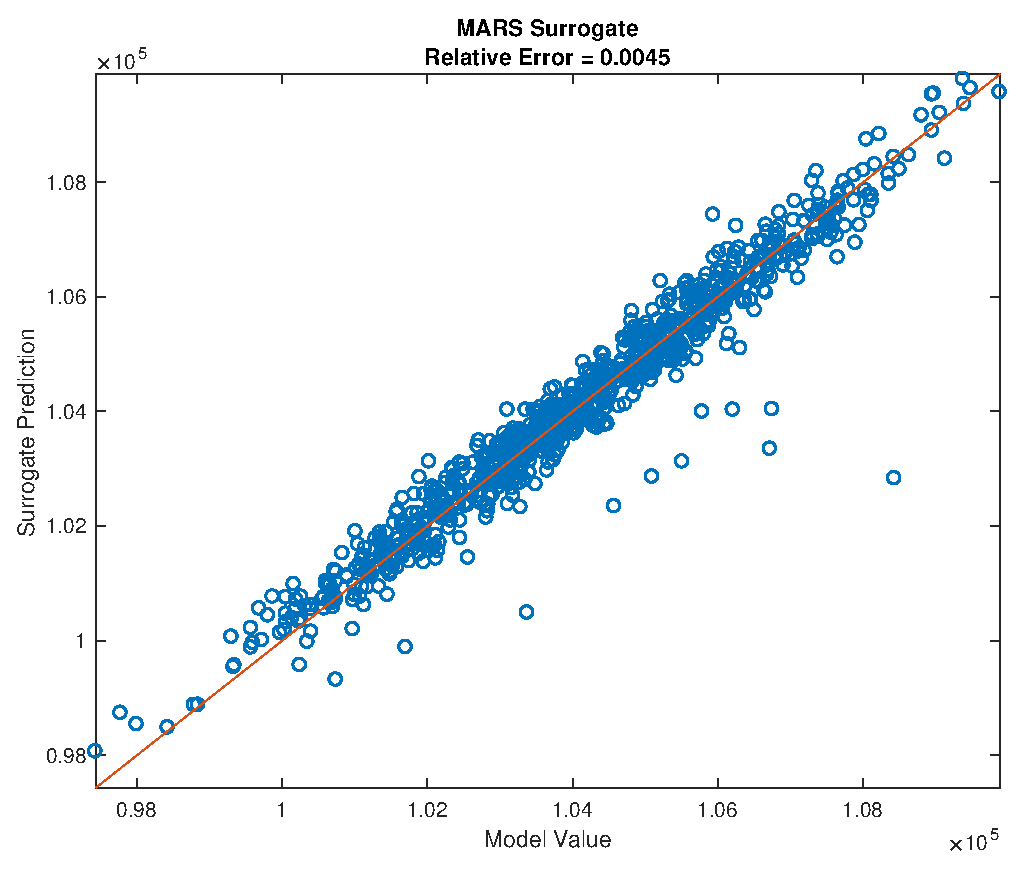
\includegraphics[width=.49 \textwidth]{Figures/K_AC_Mean_QoI_MARS_Prediction_Rectangular.eps}
\includegraphics[width=.49 \textwidth]{Figures/K_AC_Mean_QoI_MARS_VI_Rectangular.eps}
\end{figure}

Tabular data in Table~\ref{qoi_K_AC_Mean_rec}.

\begin{table}[h]
\centering
\begin{tabular}{ccccc}
Index & Identification & LR Importance & MARS Importance & MARS Ranking \\
120 & 5.5 in Buff\_e ODE & 0.2892 &  0.3871 & 1\\
121 & 1.09 in Buff\_e ODE & 0.0724 & 0.2228 & 2\\
62 & 0.143 in m4alpha and m4 beta & 0.0328 &  0.1194 & 3\\
63 &   5.67 in m4alpha and m4 beta & 0.0250 & 0.0900 & 4\\
75 & 34.9 in m6alpha & 0.0230 & 0.0550 & 5\\
61 & gKleak\_d in Neuron & 0.0188 & 0.0345 & 6\\
73 & 0.07 in J\_NMDA\_K\_d & 0.0104 & 0.0153 & 8\\
141 & z\_4 in SMCEC & 0.0099 & 0 & none\\
74 & 0.016 in m6alpha & 0.0099 & 0 & none\\
76 & 0.2 in m6alpha & 0.0083 & 0.0146 & 10\\
\end{tabular}
\caption{($K_{AC}$ Mean rectangular pulse stimulus) The importance of the parameters is assessed in two ways; ``LR Importance" is the absolute value of the linear regression coefficient normalized so that the sum of all indices equals 1 and ``MARS Importance" is delGCV measure build in MARS normalized so that the sum of all indices equals 1. The parameters are ordered according to the results from linear regression and the ordering of parameters by MARS is given in the ``MARS Ranking" column. The ``Index" column is indexing of the parameters in the code (primarily for Joey's use) and the ``Identification column" is the description of the parameter.}
\label{qoi_K_AC_Mean_rec}
\end{table}

\newpage

\subsubsection{Experimental Data Stimulus}

\begin{figure}[h]
\centering
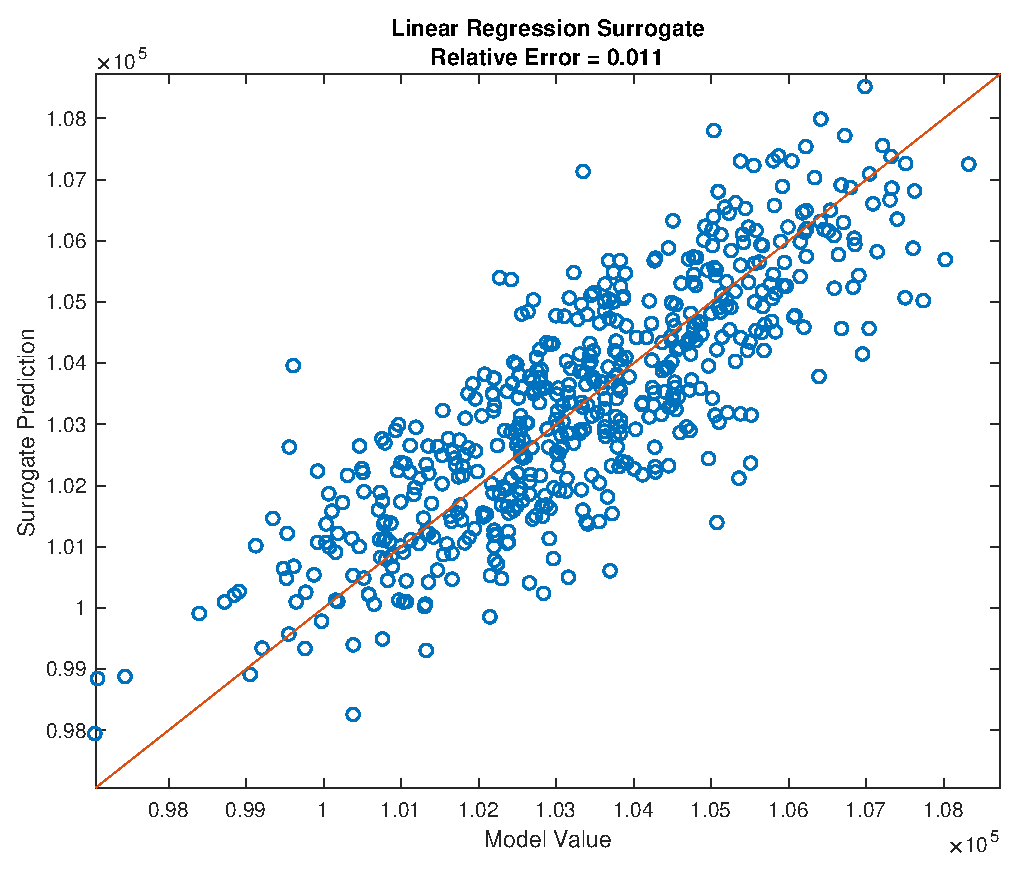
\includegraphics[width=.49 \textwidth]{Figures/K_AC_Mean_QoI_LR_Prediction_Experimental.eps}
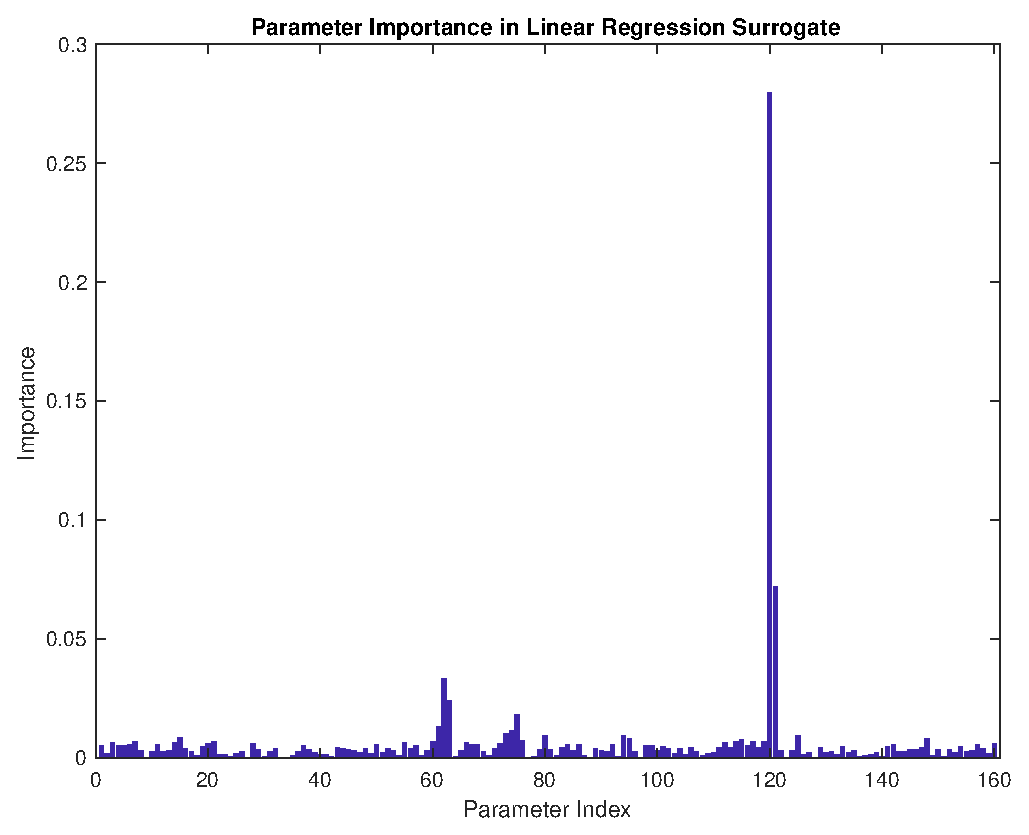
\includegraphics[width=.49 \textwidth]{Figures/K_AC_Mean_QoI_LR_VI_Experimental.eps}\\
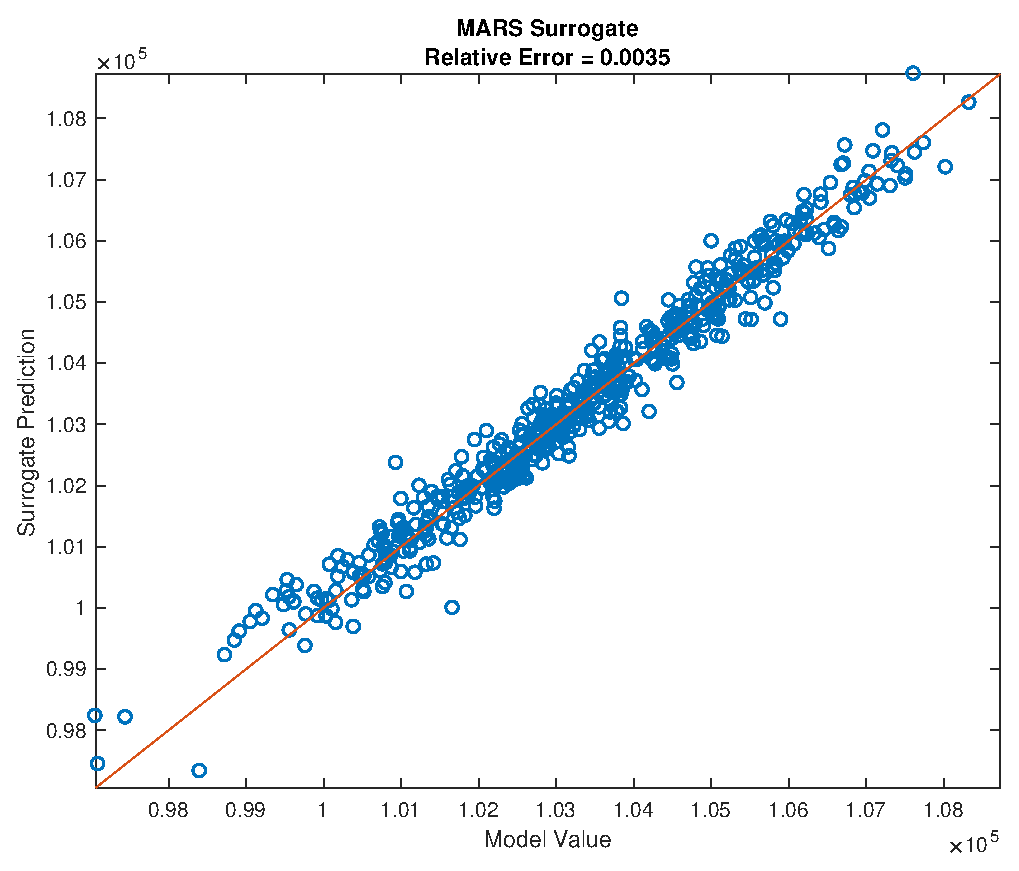
\includegraphics[width=.49 \textwidth]{Figures/K_AC_Mean_QoI_MARS_Prediction_Experimental.eps}
\includegraphics[width=.49 \textwidth]{Figures/K_AC_Mean_QoI_MARS_VI_Experimental.eps}
\end{figure}

Tabular data in Table~\ref{qoi_K_AC_Mean_ex}.

\begin{table}[h]
\centering
\begin{tabular}{ccccc}
Index & Identification & LR Importance & MARS Importance & MARS Ranking \\
120 & 5.5 in Buff\_e ODE &  0.2799 & 0.3867 & 1\\
121 & 1.09 in Buff\_e ODE & 0.0720 & 0.2413 & 2\\
62 & 0.143 in m4alpha and m4 beta & 0.0335 & 0.1141 & 3\\
63 &   5.67 in m4alpha and m4 beta &  0.0242 & 0.0805 & 4\\
75 & 34.9 in m6alpha & 0.0181 & 0.0499 & 5\\
61 & gKleak\_d in Neuron & 0.0131 & 0.0396 & 6\\
74 & 0.016 in m6alpha & 0.0114 & 0 & none\\
73 & 0.07 in J\_NMDA\_K\_d & 0.0103 & 0.0184 & 8\\
125 & v\_6 in Astrocyte & 0.0096 & 0 & none\\
94 & 34.9 in m2alpha  & 0.0093 & 0 & none\\
\end{tabular}
\caption{($K_{AC}$ Mean experimental data stimulus) The importance of the parameters is assessed in two ways; ``LR Importance" is the absolute value of the linear regression coefficient normalized so that the sum of all indices equals 1 and ``MARS Importance" is delGCV measure build in MARS normalized so that the sum of all indices equals 1. The parameters are ordered according to the results from linear regression and the ordering of parameters by MARS is given in the ``MARS Ranking" column. The ``Index" column is indexing of the parameters in the code (primarily for Joey's use) and the ``Identification column" is the description of the parameter.}
\label{qoi_K_AC_Mean_ex}
\end{table}

\newpage
\subsection{QoI \eqref{AM_AMp_Min} ($AM+AM_p$ Min)}

\subsubsection{Rectangular Pulse Stimulus}

\begin{figure}[h]
\centering
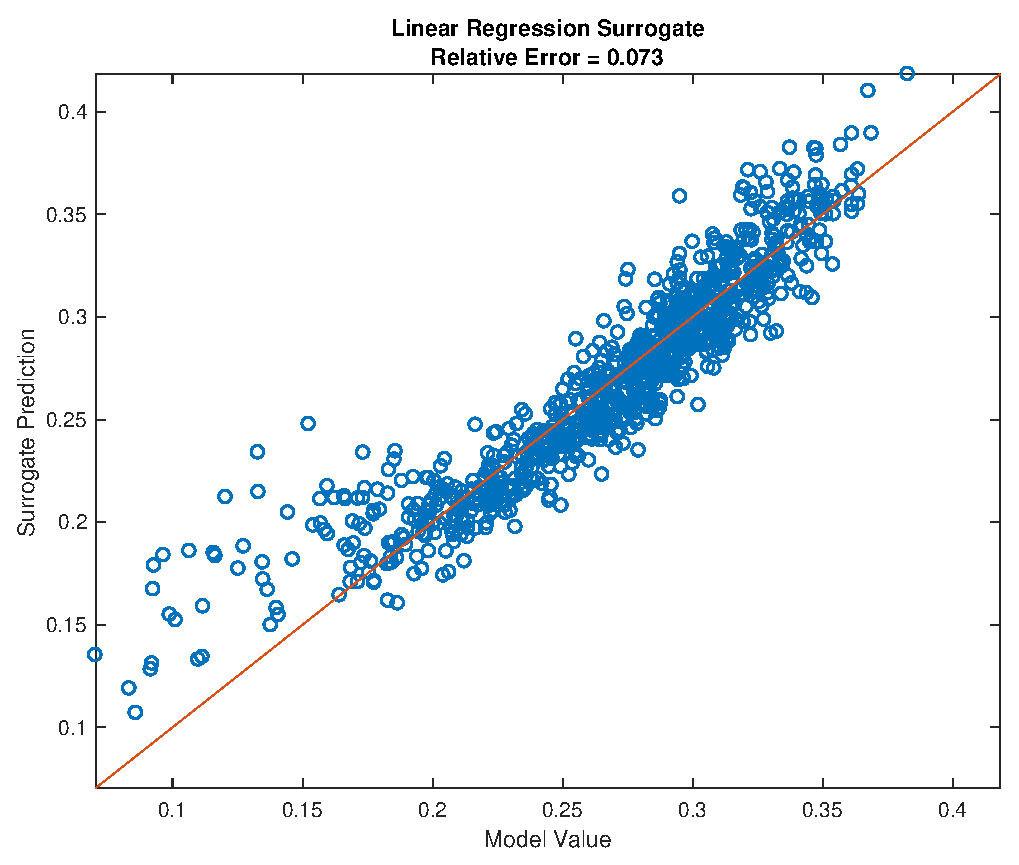
\includegraphics[width=.49 \textwidth]{Figures/AM_AMp_Min_QoI_LR_Prediction_Rectangular.eps}
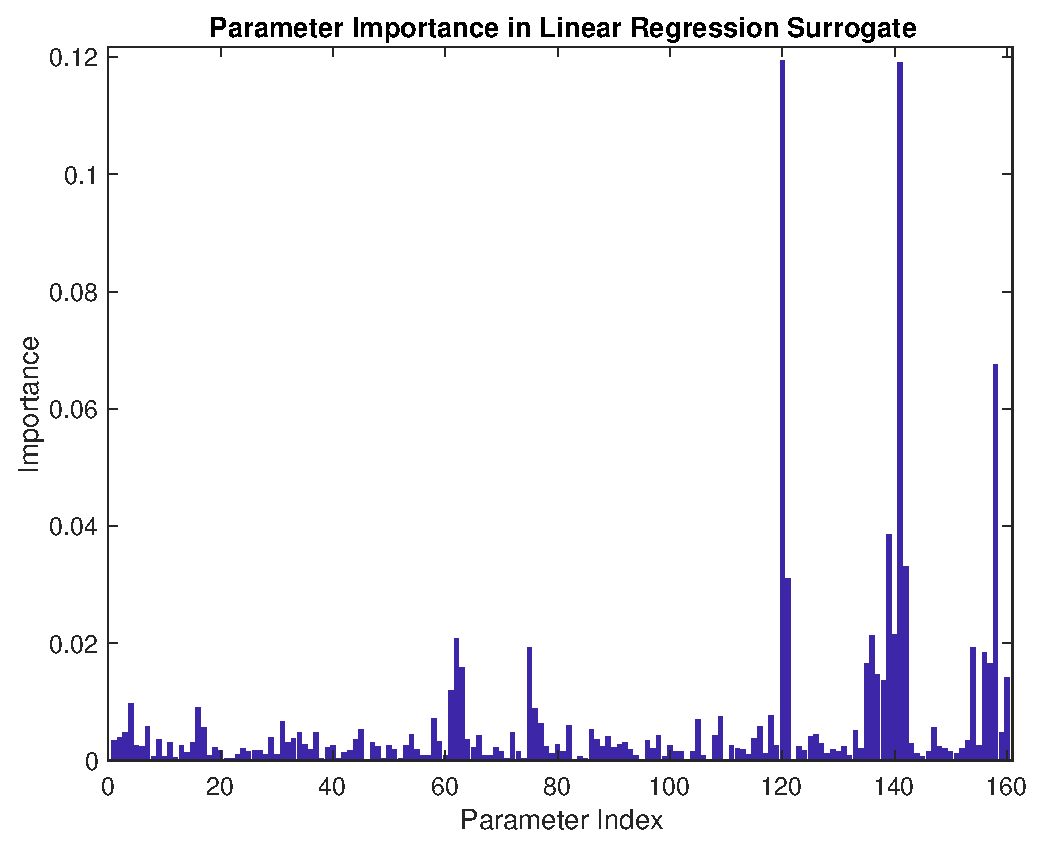
\includegraphics[width=.49 \textwidth]{Figures/AM_AMp_Min_QoI_LR_VI_Rectangular.eps}\\
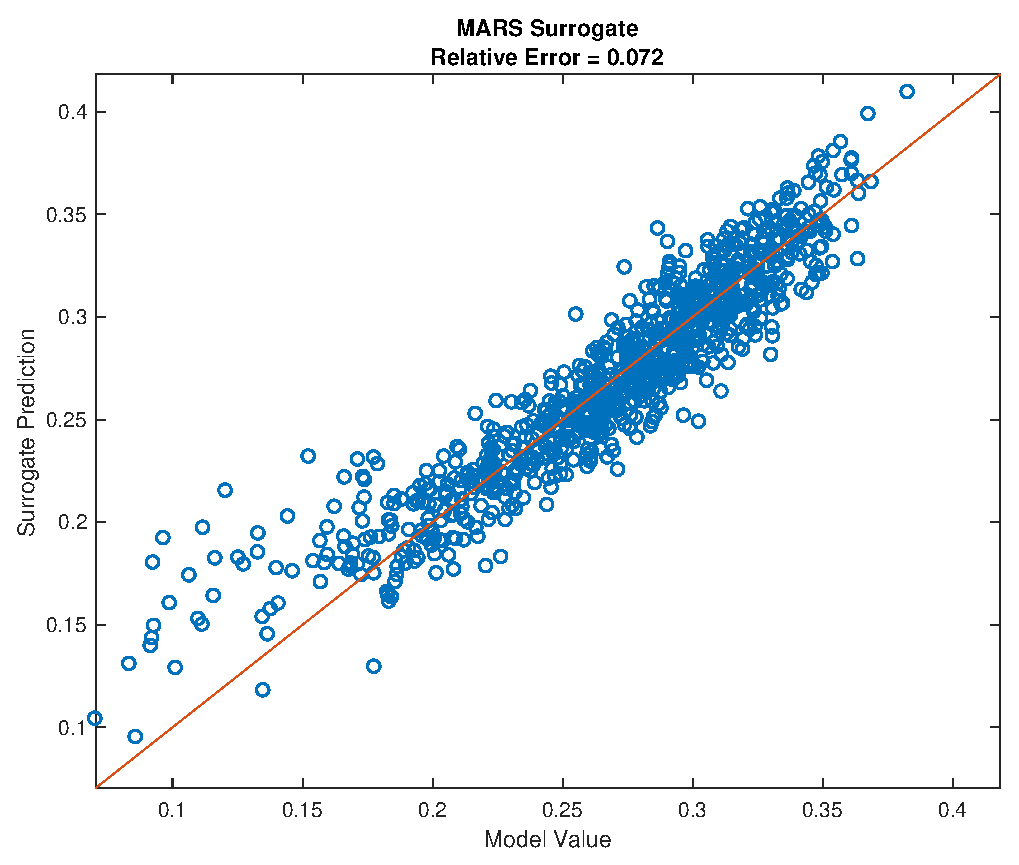
\includegraphics[width=.49 \textwidth]{Figures/AM_AMp_Min_QoI_MARS_Prediction_Rectangular.eps}
\includegraphics[width=.49 \textwidth]{Figures/AM_AMp_Min_QoI_MARS_VI_Rectangular.eps}
\end{figure}

Tabular data in Table~\ref{qoi_AM_AMp_Min_rec}.

 
\begin{table}[h]
\centering
\begin{tabular}{ccccc}
Index & Identification & LR Importance & MARS Importance & MARS Ranking \\
120 & 5.5 in Buff\_e ODE & 0.1970 & 0.0871 & 3\\
141 & z\_4 in SMCEC & 0.1005 & 0.3960 & 1\\
121 & 1.09 in Buff\_e ODE & 0.0627 & 0.0442 & 6\\
158 & n\_cross in WallMechanics & 0.0617 & 0.1801 & 2\\
139 & z\_2 in SMCEC & 0.0362 & 0.0671 & 4\\
142 & z\_5 in SMCEC & 0.0320 & 0.0503 & 5\\
140 & z\_3 in SMCEC & 0.0253 & 0.0385 & 7\\
62 & 0.143 in m4alpha and m4 beta & 0.0243 & 0.0358 & 8\\
136 & G\_K\_i in SMCEC & 0.0215 & 0.0200 & 10\\
75 & 34.9 in m6alpha & 0.0194 & 0 & none\\
\end{tabular}
\caption{($AM+AM_p$ Min rectangular pulse stimulus) The importance of the parameters is assessed in two ways; ``LR Importance" is the absolute value of the linear regression coefficient normalized so that the sum of all indices equals 1 and ``MARS Importance" is delGCV measure build in MARS normalized so that the sum of all indices equals 1. The parameters are ordered according to the results from linear regression and the ordering of parameters by MARS is given in the ``MARS Ranking" column. The ``Index" column is indexing of the parameters in the code (primarily for Joey's use) and the ``Identification column" is the description of the parameter.}
\label{qoi_AM_AMp_Min_rec}
\end{table}

\newpage

\subsubsection{Experimental Data Stimulus}

\begin{figure}[h]
\centering
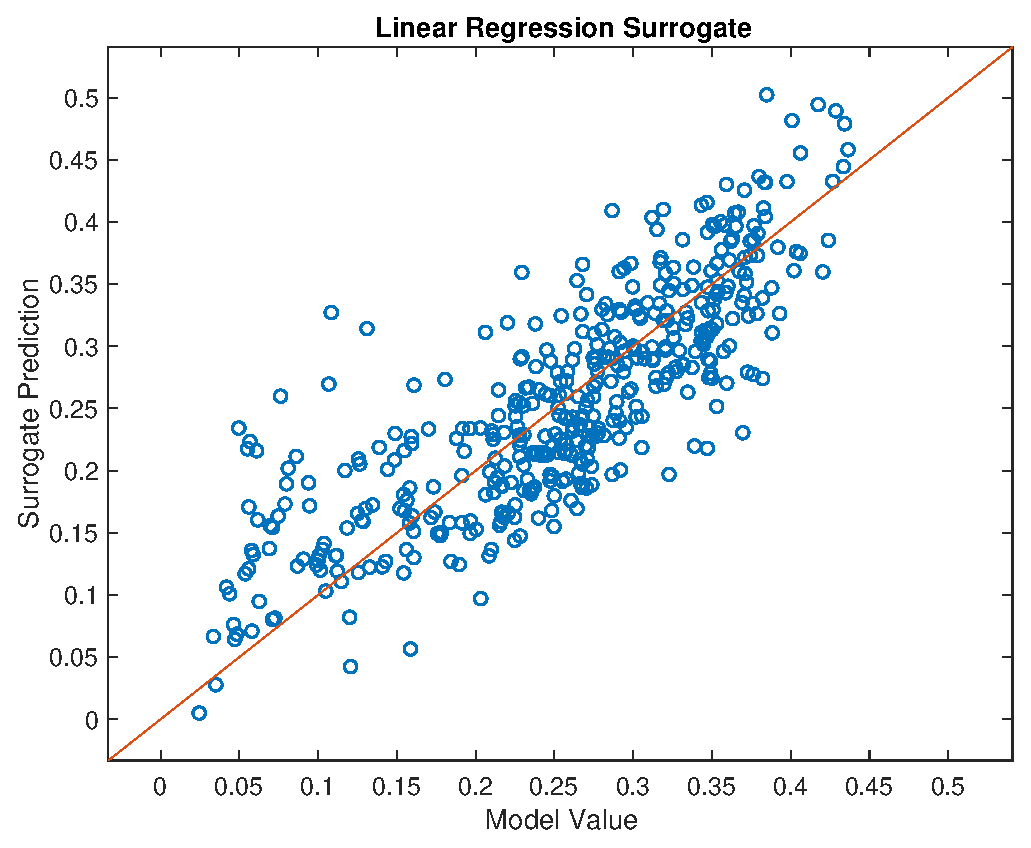
\includegraphics[width=.49 \textwidth]{Figures/AM_AMp_Min_QoI_LR_Prediction_Experimental.eps}
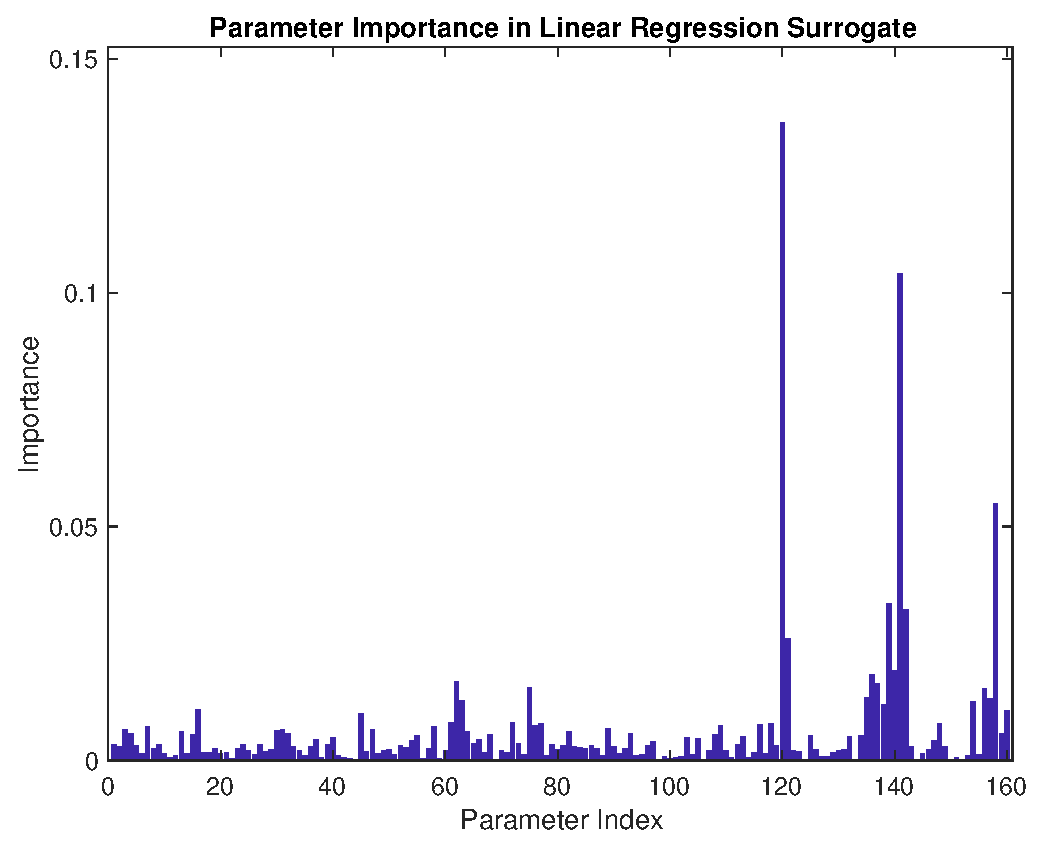
\includegraphics[width=.49 \textwidth]{Figures/AM_AMp_Min_QoI_LR_VI_Experimental.eps}\\
\includegraphics[width=.49 \textwidth]{Figures/AM_AMp_Min_QoI_MARS_Prediction_Experimental.eps}
\includegraphics[width=.49 \textwidth]{Figures/AM_AMp_Min_QoI_MARS_VI_Experimental.eps}
\end{figure}

Tabular data in Table~\ref{qoi_AM_AMp_Min_ex}.
 
\begin{table}[h]
\centering
\begin{tabular}{ccccc}
Index & Identification & LR Importance & MARS Importance & MARS Ranking \\
120 & 5.5 in Buff\_e ODE & 0.1470 & 0.0565 & 4\\
141 & z\_4 in SMCEC & 0.0783 & 0.4063 & 1\\
158 & n\_cross in WallMechanics & 0.0612 & 0.2605 & 2\\
121 & 1.09 in Buff\_e ODE & 0.0503 & 0.0312 & 6\\
139 & z\_2 in SMCEC & 0.0293 & 0.0638 & 3\\ 
142 & z\_5 in SMCEC & 0.0272 & 0.0456 & 5\\ 
94 & 34.9 in m2alpha & 0.0195 & 0 & none \\
63 &   5.67 in m4alpha and m4 beta &  0.0193 &  0.0224 & 9\\
156 & K\_7 in WallMechanics & 0.0179 & 0.0227 & 8\\
62 & 0.143 in m4alpha and m4 beta & 0.0171 & 0.0182 & 10\\
\end{tabular}
\caption{($AM+AM_p$ Min experimental data stimulus) The importance of the parameters is assessed in two ways; ``LR Importance" is the absolute value of the linear regression coefficient normalized so that the sum of all indices equals 1 and ``MARS Importance" is delGCV measure build in MARS normalized so that the sum of all indices equals 1. The parameters are ordered according to the results from linear regression and the ordering of parameters by MARS is given in the ``MARS Ranking" column. The ``Index" column is indexing of the parameters in the code (primarily for Joey's use) and the ``Identification column" is the description of the parameter.}
\label{qoi_AM_AMp_Min_ex}
\end{table}

\newpage
\subsection{QoI \eqref{AMp_Time_to_Min} ($AM_p$ Time Lag)}

\subsubsection{Rectangular Pulse Stimulus}

\begin{figure}[h]
\centering
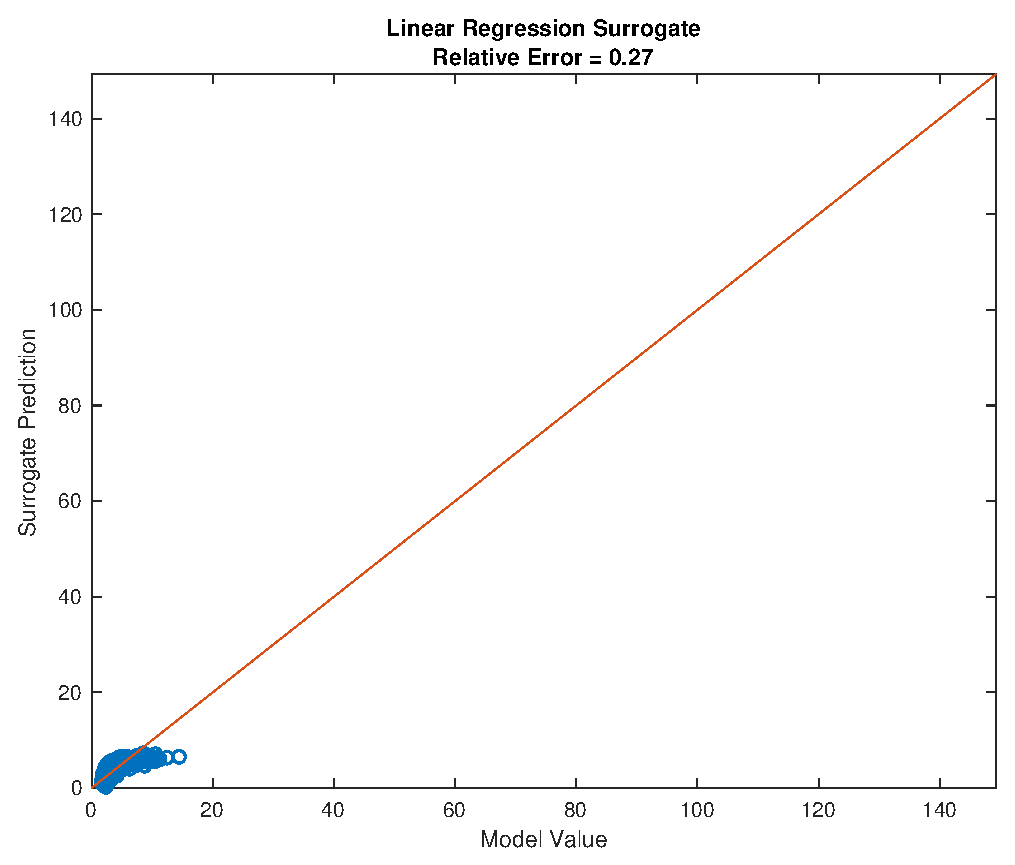
\includegraphics[width=.49 \textwidth]{Figures/AMp_Time_to_Min_QoI_LR_Prediction_Rectangular.eps}
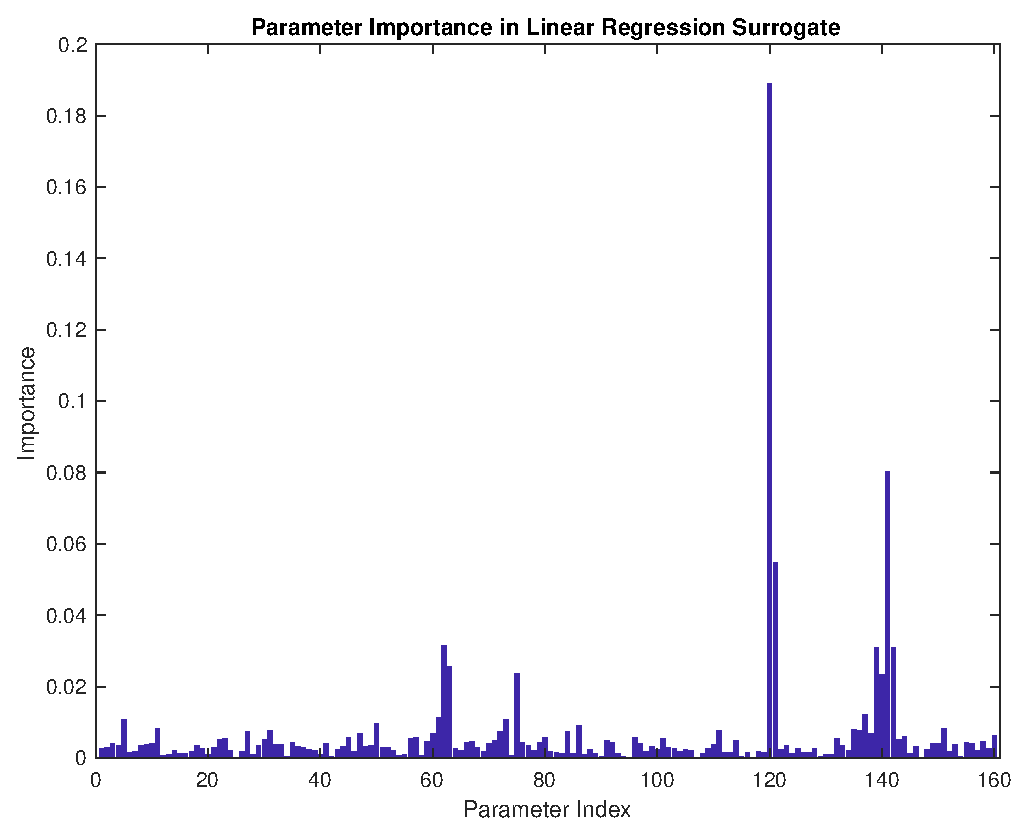
\includegraphics[width=.49 \textwidth]{Figures/AMp_Time_to_Min_QoI_LR_VI_Rectangular.eps}\\
\includegraphics[width=.49 \textwidth]{Figures/AMp_Time_to_Min_QoI_MARS_Prediction_Rectangular.eps}
\includegraphics[width=.49 \textwidth]{Figures/AMp_Time_to_Min_QoI_MARS_VI_Rectangular.eps}
\end{figure}

The surrogate model is poor, I need to work more on this QoI.

\newpage

\subsubsection{Experimental Data Stimulus}

\begin{figure}[h]
\centering
\includegraphics[width=.49 \textwidth]{Figures/AMp_Time_to_Min_QoI_LR_Prediction_Experimental.eps}
\includegraphics[width=.49 \textwidth]{Figures/AMp_Time_to_Min_QoI_LR_VI_Experimental.eps}\\
\includegraphics[width=.49 \textwidth]{Figures/AMp_Time_to_Min_QoI_MARS_Prediction_Experimental.eps}
\includegraphics[width=.49 \textwidth]{Figures/AMp_Time_to_Min_QoI_MARS_VI_Experimental.eps}
\end{figure}

The surrogate model is poor, I need to work more on this QoI.

\section{Discussion}
\section{Conclusion}
\bibliographystyle{KathisBibstyle} % no .sty!
\bibliography{library}

\end{document}